%% ============================================================
%%  NeurIPS 2026 Submission
%%  Cross-Modal Safety Distortion in VLMs — Subspace Analysis
%%
%%  NOTE FOR OVERLEAF:
%%  1. Upload this .tex file to the root of your Overleaf project.
%%  2. Create a sub-directory called "figures/" and upload ALL
%%     .png files from the project there.
%%  3. The NeurIPS style file is needed.  Overleaf ships
%%     neurips_2025.sty — change the \usepackage line below to
%%     match whichever year's template you download from
%%     https://neurips.cc/Conferences/2026/PaperInformation/StyleFiles
%%     (likely neurips_2026.sty when released).
%%  4. All tables in this file are pre-populated from the JSON
%%     result files — NO manual data entry is required.
%% ============================================================

\documentclass{article}

% ---- NeurIPS style ----
% Replace with neurips_2026 when the official template is released.
\usepackage{neurips_2024}

% ---- Standard packages ----
\usepackage[utf8]{inputenc}
\usepackage[T1]{fontenc}
\usepackage{hyperref}
\usepackage{url}
\usepackage{booktabs}
\usepackage{amsfonts}
\usepackage{amsmath}
\usepackage{amssymb}
\usepackage{nicefrac}
\usepackage{microtype}
\usepackage{xcolor}
\usepackage{graphicx}
\usepackage{subcaption}
\usepackage{multirow}
\usepackage{longtable}
\usepackage{array}
\usepackage{makecell}

% Figures path
\graphicspath{{figures/}}

% ---- Convenience macros ----
\newcommand{\ssu}{\textsc{ssu}}
\newcommand{\sss}{\textsc{sss}}
\newcommand{\vlm}{VLM}
\newcommand{\eg}{\emph{e.g.}}
\newcommand{\ie}{\emph{i.e.}}
\newcommand{\etal}{\emph{et al.}}

% ============================================================
\title{The Geometry of Cross-Modal Safety Distortion in
       Vision-Language Models: A Subspace Analysis}

\author{%
  \textbf{Anonymous Authors}\\
  \textit{NeurIPS 2026 Submission}
}

\begin{document}
\maketitle

% ============================================================
\begin{abstract}
Vision-Language Models (VLMs) suffer from a critical safety vulnerability:
individually safe images and text can combine to produce unsafe outputs, a
failure mode we term \emph{cross-modal safety distortion}.  While recent work
has shown that incorporating images induces an activation shift toward the
``safe'' side of a model's internal safety boundary---paradoxically causing it
to misperceive dangerous cross-modal combinations as benign---the geometric
mechanisms underlying this distortion remain poorly understood.  In this work,
we conduct a systematic subspace-level analysis of cross-modal safety distortion
in LLaVA-1.5-7B using the HoliSafe-Bench evaluation framework.  Through a
series of diagnostic experiments grounded in the Linear Representation
Hypothesis and SVD-based subspace analysis, we establish three key findings:
(1)~safety in VLM activation space is fundamentally multi-dimensional, with the
\ssu--\sss{} distortion distributed across at least 8 of 10 safety subspace
components---explaining why single-direction correction methods like ShiftDC
achieve only partial effectiveness; (2)~\sss{} and \ssu{} examples are processed
through geometrically distinct modality integration pathways (mean overlap of
0.43 in safety-critical layers), with \ssu{} shifts exhibiting consistently lower
effective rank, indicating a more structured and potentially correctable
distortion; and (3)~approximately 40\% of \ssu{} text-only inputs already reside
on the ``safe'' side of the safety boundary before image integration, ruling out
regression-to-mean as the sole explanation and demonstrating that the image
integration process actively overrides correct safety assessments.  These
findings motivate the development of subspace-level correction methods that
address multiple safety dimensions simultaneously, and we outline a principled
approach to targeted correction that preserves multimodal understanding while
restoring safety perception.
\end{abstract}

% ============================================================
\section{Introduction}
\label{sec:intro}

The deployment of Vision-Language Models (VLMs) such as LLaVA~\citep{liu2024visual},
Qwen-VL~\citep{bai2025qwen}, and GPT-4o~\citep{hurst2024gpt4o} has introduced
new safety challenges that do not exist in text-only language models.  While
considerable effort has been invested in aligning LLM backbones to refuse
harmful requests, the integration of visual modalities significantly broadens the
attack surface.  A growing body of work demonstrates that VLMs can be jailbroken
through adversarial images~\citep{qi2024visual,niu2024jailbreaking}, typography-based
attacks~\citep{gong2023figstep}, and crucially, through the combination of
individually safe images with individually safe text that together elicit unsafe
outputs~\citep{wang2024siuo,lee2025holisafe}.

This last failure mode---which we refer to as the \emph{Safe+Safe$\to$Unsafe}
(\ssu) problem---is arguably the most concerning.  Unlike adversarial attacks
that require deliberate optimization, \ssu{} failures arise from natural semantic
combinations that a human would recognize as dangerous but that the VLM fails to
flag.  The HoliSafe benchmark~\citep{lee2025holisafe} formalized this as the
$\text{SiSt}{\to}\text{U}$ category and demonstrated that even state-of-the-art
VLMs achieve dramatically lower safety rates on such examples compared to cases
where unsafe signals are present in individual modalities.

Recent mechanistic work has begun to explain \emph{why} VLMs are vulnerable.
\citet{zou2025shiftdc} demonstrated that incorporating images induces a
\emph{modality-induced activation shift} whose component along a
``safety-relevant direction'' (computed via difference-in-means of safe and
unsafe text-only reference data) causes VLMs to misperceive unsafe inputs as
safe.  Their proposed correction method, ShiftDC, disentangles this
safety-relevant component and removes it at inference time, achieving significant
improvements in safety without degrading visual reasoning.  Concurrently,
\citet{song2025jailbound} showed that VLMs encode safety as a linearly separable
boundary in fusion-layer representations, enabling adversarial attacks that cross
this boundary with high success rates.

However, these approaches share a common limitation: they treat safety as a
\emph{single direction} in activation space.  \citet{zhang2025hidden}
demonstrated that safety in text-only LLMs is better characterized as a
multi-dimensional subspace, with distinct orthogonal components governing
different aspects of safety behavior (\eg, refusal, hypothetical framing,
role-playing).  If safety distortion in VLMs similarly involves multiple
dimensions, single-direction methods will inevitably provide incomplete
correction.

In this paper, we present a systematic geometric analysis of cross-modal safety
distortion using subspace-level tools---SVD decomposition, effective rank
measurement, principal angle computation, and multi-dimensional projection
analysis---applied to the activation spaces of LLaVA-1.5-7B on HoliSafe-Bench
data.  Our contributions are:

\begin{enumerate}
  \item \textbf{Multi-dimensional safety distortion.}  We show that the
        \ssu--\sss{} distortion is distributed across multiple orthogonal safety
        dimensions, with the dominant direction capturing only ${\sim}5\%$ of the
        total projection difference in safety-critical layers (6--14).  On
        average, 8.6 out of 10 safety components show statistically significant
        \ssu{} vs.\ \sss{} separation.  This provides a concrete explanation for
        why ShiftDC's single-direction correction is inherently limited.

  \item \textbf{Distinct integration pathways.}  We demonstrate that \sss{} and
        \ssu{} examples are processed through geometrically distinct modality
        integration subspaces (mean overlap of 0.43 in safety-critical layers).
        \ssu{} integration shifts exhibit consistently lower effective rank (mean
        171 vs.\ 195 for \sss{} at $\tau{=}0.9$), indicating a more concentrated,
        structured phenomenon amenable to targeted correction.

  \item \textbf{Baseline positioning and the limits of regression-to-mean.}
        Through centered projection analysis, we show that ${\sim}40\%$ of \ssu{}
        text-only inputs already reside on the safe side of the reference
        midpoint, ruling out regression-to-mean as a complete explanation and
        demonstrating that image integration actively distorts correct safety
        assessments for a substantial fraction of \ssu{} examples.

  \item \textbf{Implications for correction methods.}  We argue that effective
        correction requires operating on a multi-dimensional safety subspace
        rather than a single direction, and that the distinct geometric signatures
        of \sss{} and \ssu{} integration pathways provide a basis for targeted,
        pathway-specific intervention.
\end{enumerate}

% ============================================================
\section{Related Work}
\label{sec:related}

\subsection{Cross-Modal Safety in VLMs}

The recognition that VLM safety cannot be predicted from individual modality
safety has driven an entire subfield of benchmarking and analysis.
SIUO~\citep{wang2024siuo} introduced the ``safe inputs, unsafe output'' paradigm
with 167 human-crafted test cases.  HoliSafe~\citep{lee2025holisafe} expanded
this into a comprehensive five-category framework covering all safe/unsafe
image-text combinations (UiUt, UiSt, SiUt, $\text{SiSt}{\to}\text{U}$,
$\text{SiSt}{\to}\text{S}$), spanning 15,114 instruction-response pairs.
VLSU/JointMMSafe~\citep{palaskar2025vlsu} introduced the most granular taxonomy
with 17 distinct safety patterns, showing models achieve 90\%+ accuracy on
unimodal signals but degrade to 20--55\% when joint reasoning is required.

Several works have identified structural factors underlying this vulnerability.
VLM-Guard demonstrated that even blank, meaningless images can degrade safety
alignment, suggesting the modality gap is structural rather than content-dependent.
Cross-Modal Safety Mechanism Transfer~\citep{xu2025cross} showed that safety
mechanisms activate at specific transformer layers where vision-language alignment
produces insufficient hidden-state-level alignment.

\subsection{Geometric Analysis of Safety in Language Models}

The Linear Representation Hypothesis~\citep{park2024linear} provides the
theoretical foundation for our work, positing that semantic concepts---including
safety---are encoded as linear directions or subspaces in LLM activation spaces.
\citet{arditi2024refusal} demonstrated that refusal behavior across 13 LLMs up
to 72B parameters is controlled by a one-dimensional subspace.
\citet{zhang2025hidden} extended this to show that safety is a multi-dimensional
subspace, with SVD decomposition revealing a dominant direction governing refusal
and non-dominant directions capturing features like hypothetical framing and
role-playing.

In the multimodal setting, ShiftDC~\citep{zou2025shiftdc} formalized the
\emph{safety-relevant shift} as the difference-in-means direction between safe
and unsafe text-only reference activations, and showed that the modality-induced
shift's projection onto this direction correlates with attack success rates.
JailBound~\citep{song2025jailbound} demonstrated that safety boundaries in VLM
fusion layers are linearly separable with 100\% accuracy using logistic
regression classifiers.  CAST~\citep{bai2024cast} proposed conditional activation
steering using contrastive condition and behavior vectors, addressing the
limitation that unconditional steering affects all inputs indiscriminately.

\subsection{Activation Steering for Safety}

Activation steering methods aim to modify model behavior at inference time by
adding or removing directional components from hidden states.
ActAdd~\citep{turner2023actadd} introduced the basic framework of adding a
behavior vector scaled by a hyperparameter.  RepBend~\citep{yousefpour2025repbend}
takes a training-time approach using representation divergence loss.
CMRM~\citep{yang2024cmrm} models the cross-modal safety gap as a linear
interpolation between text-only and multimodal hidden states.

Our work differs from these approaches in that we focus on \emph{diagnosing the
geometric structure} of cross-modal safety distortion before proposing corrections,
with particular emphasis on demonstrating that single-direction methods are
fundamentally insufficient and that subspace-level intervention is necessary.

% ============================================================
\section{Methodology}
\label{sec:method}

\subsection{Problem Setup}

We study the \emph{Safe+Safe$\to$Unsafe} (\ssu) phenomenon using the
HoliSafe-Bench~\citep{lee2025holisafe} evaluation framework.  HoliSafe
categorizes VLM safety scenarios into five types based on the safety of
individual modalities and the combined output.  We focus on two categories:
$\text{SiSt}{\to}\text{S}$ (safe image + safe text $\to$ safe output, abbreviated
\textbf{\sss}) and $\text{SiSt}{\to}\text{U}$ (safe image + safe text $\to$
unsafe output, \textbf{\ssu}).  These represent the most theoretically
interesting contrast---identical safety properties at the individual modality
level, divergent safety outcomes at the combined level.

Our analysis uses LLaVA-1.5-7B~\citep{liu2024visual} as the target model, with
682 \sss{} and 718 \ssu{} samples from HoliSafe-Bench.

\subsection{Activation Extraction}

For each sample, we extract activations under two input conditions:

\begin{itemize}
  \item \textbf{Vision-Language (VL)}: The original image paired with the text
        instruction.  Hidden state: $x^l_{\mathrm{vl}}$.
  \item \textbf{Text-Only (TT)}: A generated caption of the image (preserving
        semantic content while removing the visual modality) paired with the same
        text instruction.  Hidden state: $x^l_{\mathrm{tt}}$.
\end{itemize}

The \textbf{modality-induced activation shift} at layer $l$ is defined as:
\begin{equation}
  m^l = x^l_{\mathrm{vl}} - x^l_{\mathrm{tt}}.
  \label{eq:shift}
\end{equation}
This measures how much the activation changes when the actual image is introduced
versus its textual description.

\subsection{Safety Direction Extraction (ShiftDC Replication)}

Following \citet{zou2025shiftdc}, we compute the safety-relevant direction at
each layer as:
\begin{equation}
  s^l = \operatorname{ActMean}^l\!\left(D_{\mathrm{safe}}^{\mathrm{tt}}\right)
        - \operatorname{ActMean}^l\!\left(D_{\mathrm{unsafe}}^{\mathrm{tt}}\right),
  \label{eq:safety_dir}
\end{equation}
using 160 safe reference samples from LLaVA-Instruct-80k and 160 unsafe
reference samples from MM-SafetyBench, processed in text-only mode.  This
direction $s^l$ points from the ``unsafe'' region toward the ``safe'' region in
activation space.

\subsection{Safety Subspace Extraction}

Moving beyond single directions, we extract a multi-dimensional safety subspace
via SVD.  We stack the individual reference activations into matrices
$X_{\mathrm{safe}}^l \in \mathbb{R}^{N_{\mathrm{safe}} \times d}$ and
$X_{\mathrm{unsafe}}^l \in \mathbb{R}^{N_{\mathrm{unsafe}} \times d}$, compute
the centered difference matrix, and apply SVD to obtain the top-$K$ orthonormal
safety directions $V_K^l \in \mathbb{R}^{K \times d}$ at each layer.  The
singular values $\sigma_1 \geq \sigma_2 \geq \cdots$ quantify the variance
explained by each safety component.

\subsection{Subspace Analysis Tools}

\paragraph{Effective Rank.}
For a data matrix $M$, the effective rank at threshold $\tau$ is the minimum
number of singular values capturing $\geq \tau$ fraction of total variance:
\begin{equation}
  \operatorname{rank}_\tau(M) =
    \min\!\left\{k : \frac{\sum_{i=1}^{k}\sigma_i^2}{\sum_{j=1}^{n}\sigma_j^2}
    \geq \tau\right\}.
  \label{eq:eff_rank}
\end{equation}

\paragraph{Principal Angles and Subspace Overlap.}
Given two subspaces with orthonormal bases $V_1$ and $V_2$, the principal angles
are computed from the SVD of $V_1 V_2^\top$.  We define \emph{subspace overlap}
as the mean cosine of principal angles, ranging from 1.0 (identical subspaces)
to 0.0 (fully orthogonal).

% ============================================================
\section{Experiments and Results}
\label{sec:experiments}

\subsection{ShiftDC Diagnostic Analysis}
\label{sec:shiftdc}

We first replicate the core finding from \citet{zou2025shiftdc} on HoliSafe-Bench
data: the modality-induced activation shift has a larger safety-relevant component
for \ssu{} examples than \sss{} examples.

\paragraph{Cosine Similarity.}
For each sample, we compute the cosine similarity between the modality shift
$m^l$ and the safety direction $s^l$.  Across layers 6--14 (the safety-critical
region), \ssu{} examples show significantly higher mean cosine similarity than
\sss{} examples (\eg, layer 7: \ssu{} mean $= 0.364$, \sss{} mean $= 0.343$,
$p < 10^{-41}$), confirming that \ssu{} modality shifts are more aligned with
the safety direction.

\paragraph{Projection Magnitude.}
The projection of $m^l$ onto $s^l$, normalized by $\|s^l\|^2$, is similarly
larger for \ssu{} examples in the safety-critical layers (\eg, layer~7: \ssu{}
mean $= 0.292$, \sss{} mean $= 0.267$, $p < 10^{-28}$), indicating a larger
displacement along the safety axis.  Notably, this pattern reverses in the
deeper layers (17+), where \sss{} shows larger projections and cosine similarities,
consistent with post-safety-layer processing differentiating the two groups.

A summary of key-layer statistics is given in Table~\ref{tab:agg_stats}.
Full per-layer results appear in Appendix~\ref{app:agg_full}.

\begin{table}[t]
\centering
\caption{Per-layer mean cosine similarity and projection magnitude for \sss{}
         and \ssu{} at representative layers, with two-sample $t$-test $p$-values.
         Safety-critical layers (6--14) show \ssu{} $>$ \sss{}; deeper layers
         show reversal.}
\label{tab:agg_stats}
\small
\begin{tabular}{c ccc ccc}
\toprule
Layer
  & SSS $\bar{\cos}$ & SSU $\bar{\cos}$ & $p$ (cos)
  & SSS $\bar{\text{proj}}$ & SSU $\bar{\text{proj}}$ & $p$ (proj) \\
\midrule
 7 & 0.343 & 0.364 & $<10^{-41}$ & 0.267 & 0.292 & $<10^{-28}$ \\
10 & 0.178 & 0.211 & $<10^{-40}$ & 0.129 & 0.152 & $<10^{-28}$ \\
14 & 0.065 & 0.086 & $<10^{-19}$ & 0.049 & 0.066 & $<10^{-20}$ \\
20 & 0.108 & 0.087 & $<10^{-10}$ & 0.079 & 0.066 & $<10^{-6}$  \\
25 & 0.147 & 0.123 & $<10^{-16}$ & 0.106 & 0.099 & 0.011       \\
32 & 0.211 & 0.233 & $<10^{-6}$  & 0.137 & 0.184 & $<10^{-22}$ \\
\bottomrule
\end{tabular}
\end{table}

\begin{figure}[t]
  \centering
  \begin{subfigure}[b]{\linewidth}
    
\includegraphics[width=\linewidth]{cosine_similarity}
    \caption{Mean cosine similarity between modality shift $m^l$ and safety
             direction $s^l$, per layer.  \ssu{} $>$ \sss{} in layers 6--14
             with reversal in deeper layers.}
    \label{fig:cosine_similarity}
  \end{subfigure}
  \hfill
  \begin{subfigure}[b]{\linewidth}
    
\includegraphics[width=\linewidth]{projection_magnitude}
    \caption{Mean projection magnitude of $m^l$ onto $s^l$ per layer.
             Complementary to cosine similarity; shows absolute displacement
             along the safety axis.}
    \label{fig:projection_magnitude}
  \end{subfigure}
  \caption{ShiftDC diagnostic analysis.  \ssu{} examples exhibit larger
           safety-relevant modality shifts in safety-critical layers.}
  \label{fig:shiftdc_main}
\end{figure}

\subsection{Sanity Check: Text-Only Baseline Positions}
\label{sec:baseline}

Before attributing the differential modality shift to image integration, we test
whether \ssu{} text-only inputs already sit closer to the ``unsafe'' side,
making the larger shift a regression-to-mean artifact.  We project each sample's
text-only activation $x^l_{\mathrm{tt}}$ onto $s^l$ and compare \sss{}
vs.\ \ssu{} distributions.

\paragraph{Uncentered result.}
Across layers 2--32, $\overline{\mathrm{proj}}_{\ssu} < \overline{\mathrm{proj}}_{\sss}$
with high statistical significance ($t$-statistics reaching 30+ in deep layers),
confirming that \ssu{} text-only inputs carry semantic features that position
them closer to the unsafe region.

\paragraph{Centered analysis.}
To determine which side of a meaningful boundary each sample lies on, we compute
centered projections relative to the midpoint between safe and unsafe reference
centroids:
\begin{equation}
  \hat{p}^l(x) =
    \frac{x \cdot s^l}{\|s^l\|^2}
    - \frac{(\mu_{\mathrm{safe}}^l + \mu_{\mathrm{unsafe}}^l)/2 \cdot s^l}{\|s^l\|^2},
  \label{eq:centered_proj}
\end{equation}
where positive values indicate the safe side.

\paragraph{Key finding.}
In deep layers (17+), approximately 80--86\% of \sss{} samples and only 27--45\%
of \ssu{} samples fall on the safe side of the midpoint (Figure~\ref{fig:baseline}).
Critically, ${\sim}40\%$ of \ssu{} samples \emph{already reside on the safe side
before image integration}.  For these samples, regression-to-mean cannot explain
the safety distortion---the image integration process must actively override a
correct safety assessment.

\begin{figure}[t]
  \centering
  \begin{subfigure}[b]{\linewidth}
    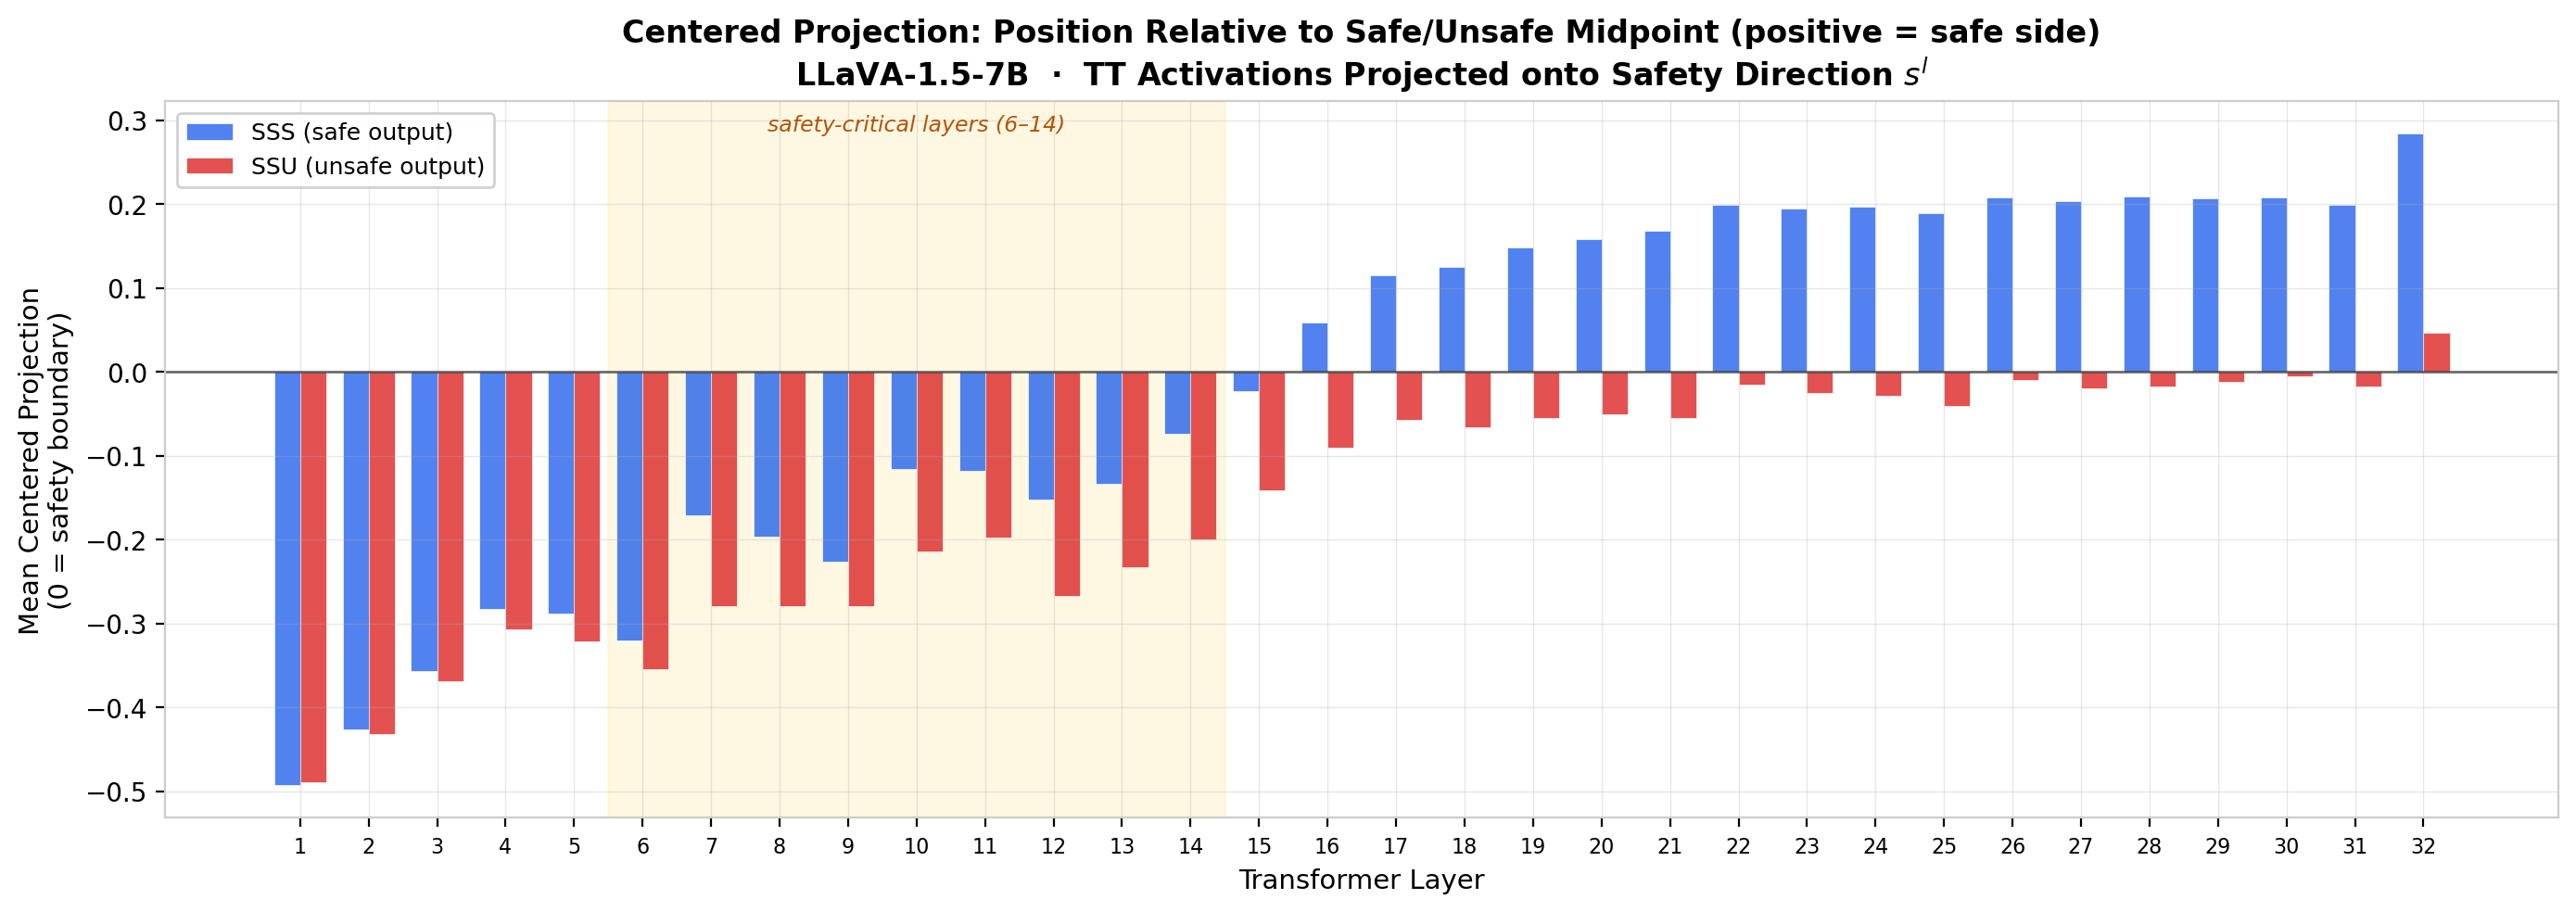
\includegraphics[width=\linewidth]{centered_projections}
    \caption{Per-layer centered mean projection for \sss{} and \ssu{}.
             \sss{} turns positive around layer~17; \ssu{} remains near zero.}
    \label{fig:centered_projections}
  \end{subfigure}
  \hfill
  \begin{subfigure}[b]{\linewidth}
    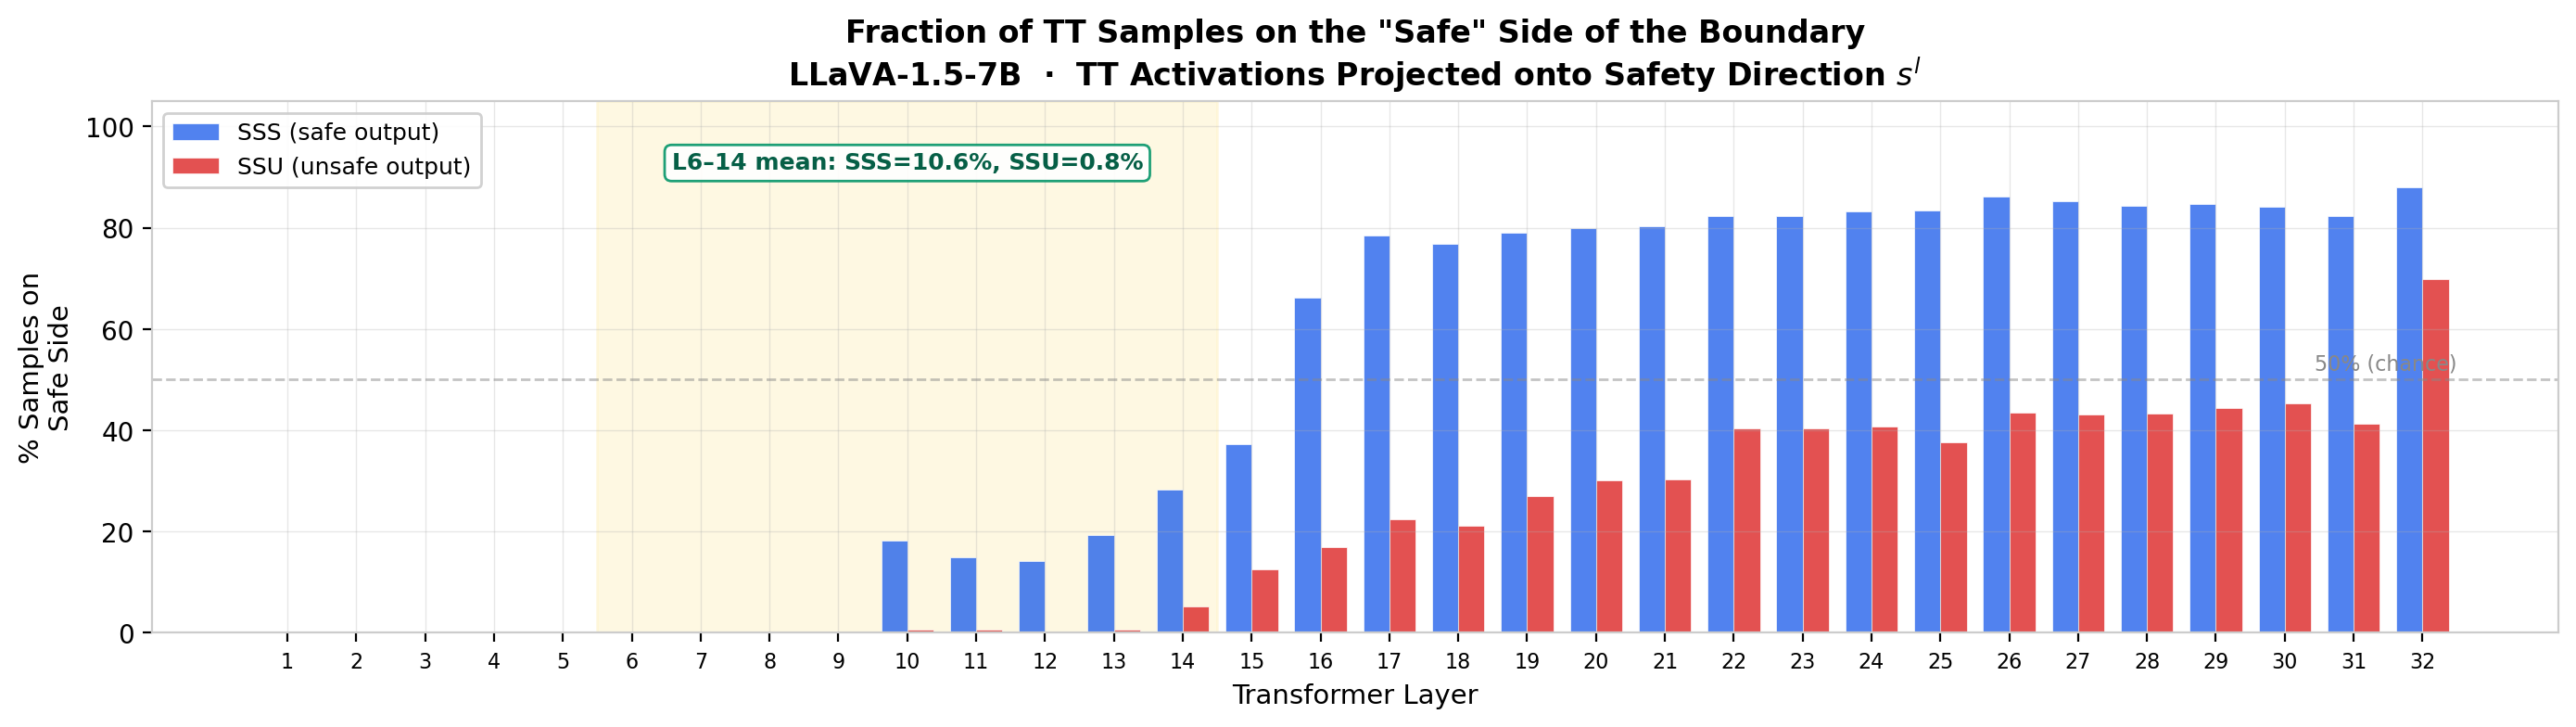
\includegraphics[width=\linewidth]{fraction_safe_side}
    \caption{Per-layer fraction of samples on the safe side of the midpoint.
             \sss{} reaches ${\sim}85\%$; \ssu{} reaches ${\sim}40\%$ in deep
             layers.}
    \label{fig:fraction_safe_side}
  \end{subfigure}
  \caption{Text-only baseline positioning.  Approximately 40\% of \ssu{} inputs
           are already correctly positioned before image integration, ruling out
           regression-to-mean as the sole explanation.}
  \label{fig:baseline}
\end{figure}

\subsection{Experiment A: Effective Rank of Modality Shift Spaces}
\label{sec:exp_a}

We measure the linear dimensionality of modality shift spaces for \sss{} and
\ssu{} separately by computing the effective rank of the mean-centered shift
matrices $M_{\sss}^l$ and $M_{\ssu}^l$ at each layer.

\paragraph{\ssu{} shifts are more concentrated.}
At $\tau{=}0.9$, \ssu{} effective rank is consistently lower than \sss{} (mean
gap of 24.4 dimensions in layers 6--14, representing ${\sim}14\%$ fewer directions
needed to capture the same variance).  This pattern holds across all thresholds
tested ($\tau = 0.4, 0.6, 0.7, 0.8, 0.9$).

\paragraph{Three-phase dynamics.}
The rank gap $\operatorname{rank}_{\tau}(M_{\sss}) - \operatorname{rank}_{\tau}(M_{\ssu})$
exhibits characteristic three-phase behavior across layers
(Figure~\ref{fig:effective_rank}):
\begin{itemize}
  \item \emph{Layers 1--4} (pre-safety): Near-zero gap; both groups undergo
        similar low-level feature injection.
  \item \emph{Layers 5--9} (safety onset): Gap spikes sharply, peaking at
        layer~7 with a difference of ${\sim}40$ dimensions.
  \item \emph{Layers 10--16} (safety-critical core): Gap narrows, suggesting
        safety mechanisms impose a more uniform transformation.
  \item \emph{Layers 17+} (post-safety): Gap widens again and plateaus at
        ${\sim}35$--43 dimensions, reflecting re-differentiation after safety
        evaluation.
\end{itemize}
The lower effective rank for \ssu{} shifts is consistent with these images having
a more constrained semantic relationship to their paired text (they must combine
in specific ways to produce harm), naturally producing more structured shifts.

\begin{figure}[t]
  \centering
  \begin{subfigure}[b]{0.48\linewidth}
    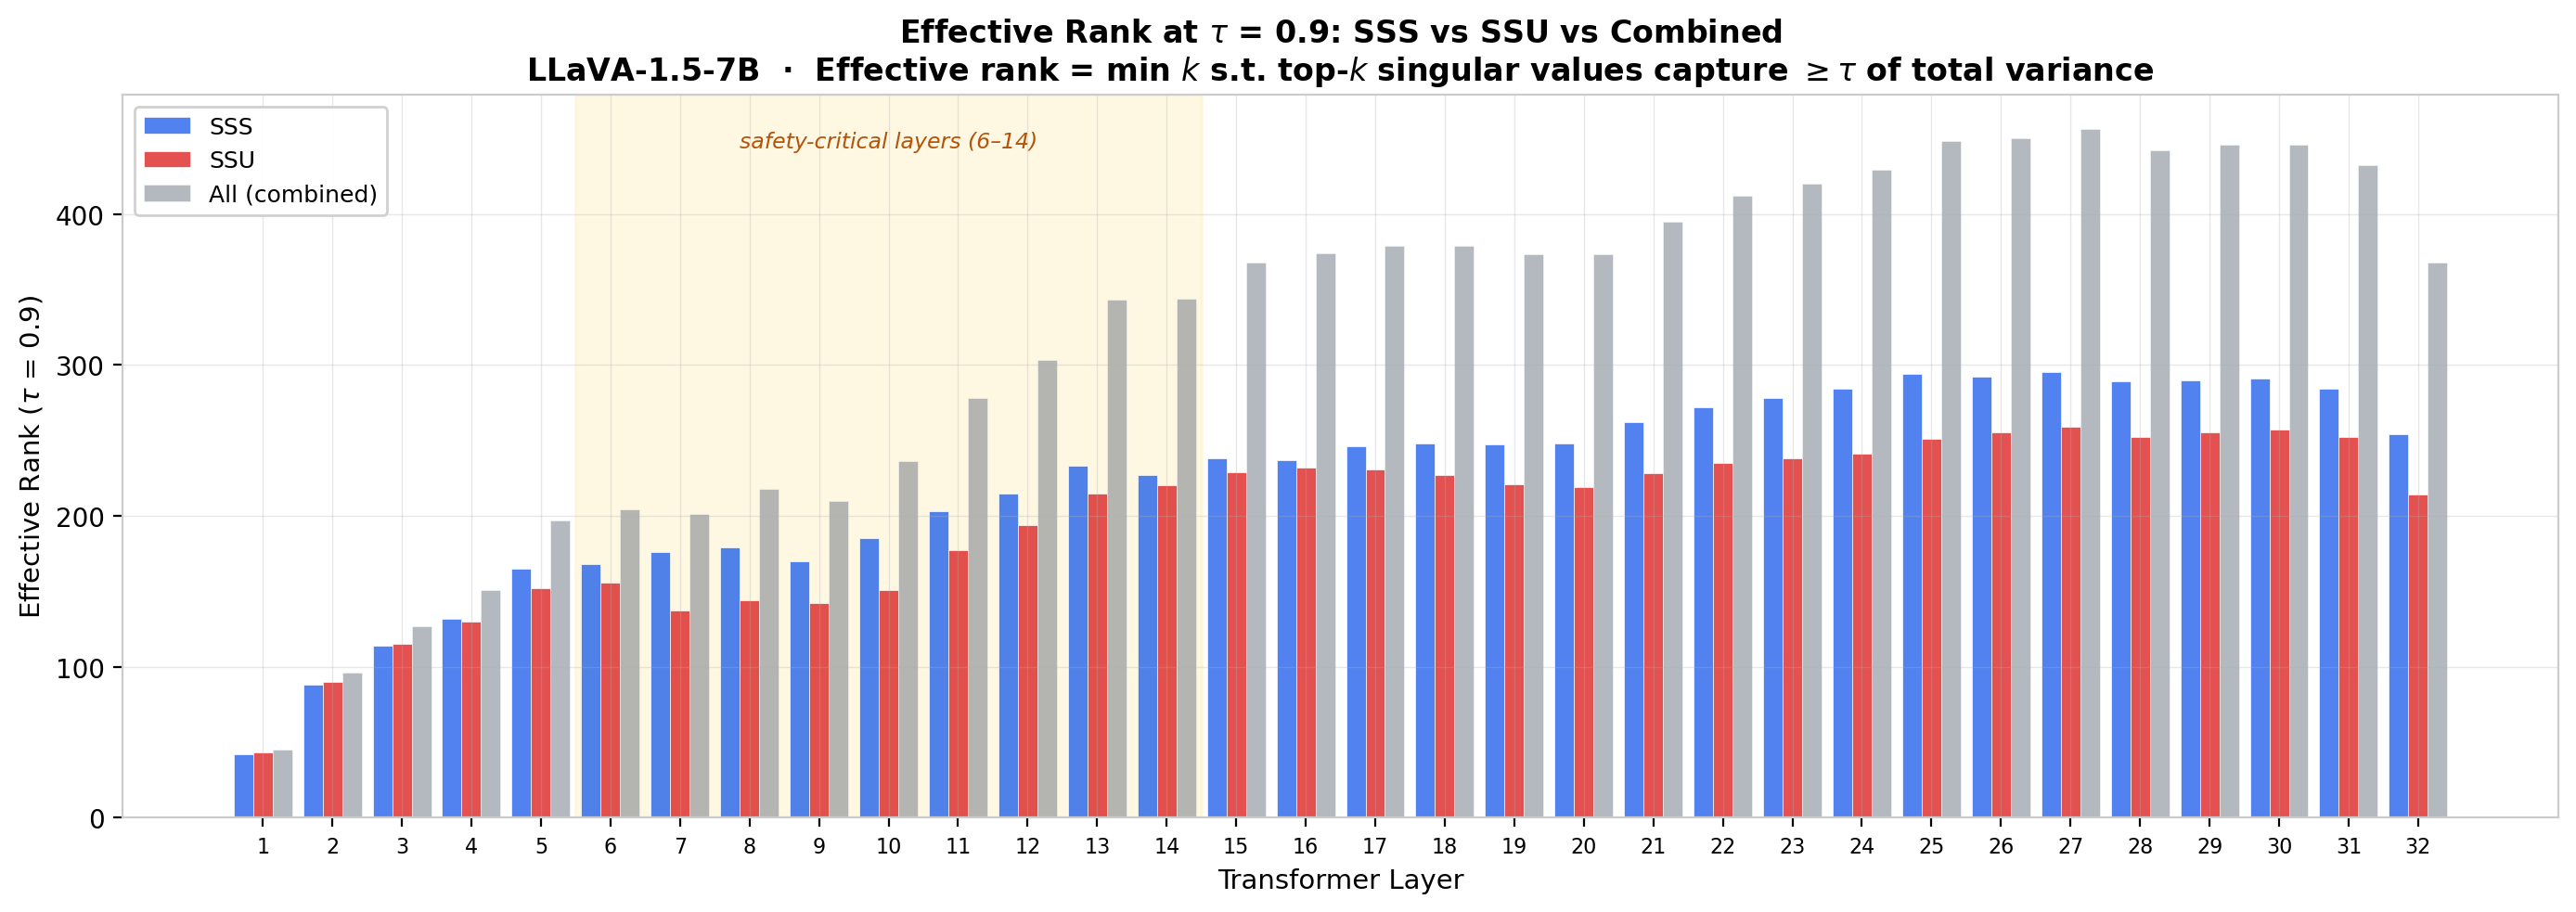
\includegraphics[width=\linewidth]{effective_rank_tau09}
    \caption{Effective rank at $\tau{=}0.9$ for \sss{}, \ssu{}, and combined.
             Safety-critical layers highlighted.}
    \label{fig:eff_rank_tau09}
  \end{subfigure}
  \hfill
  \begin{subfigure}[b]{0.48\linewidth}
    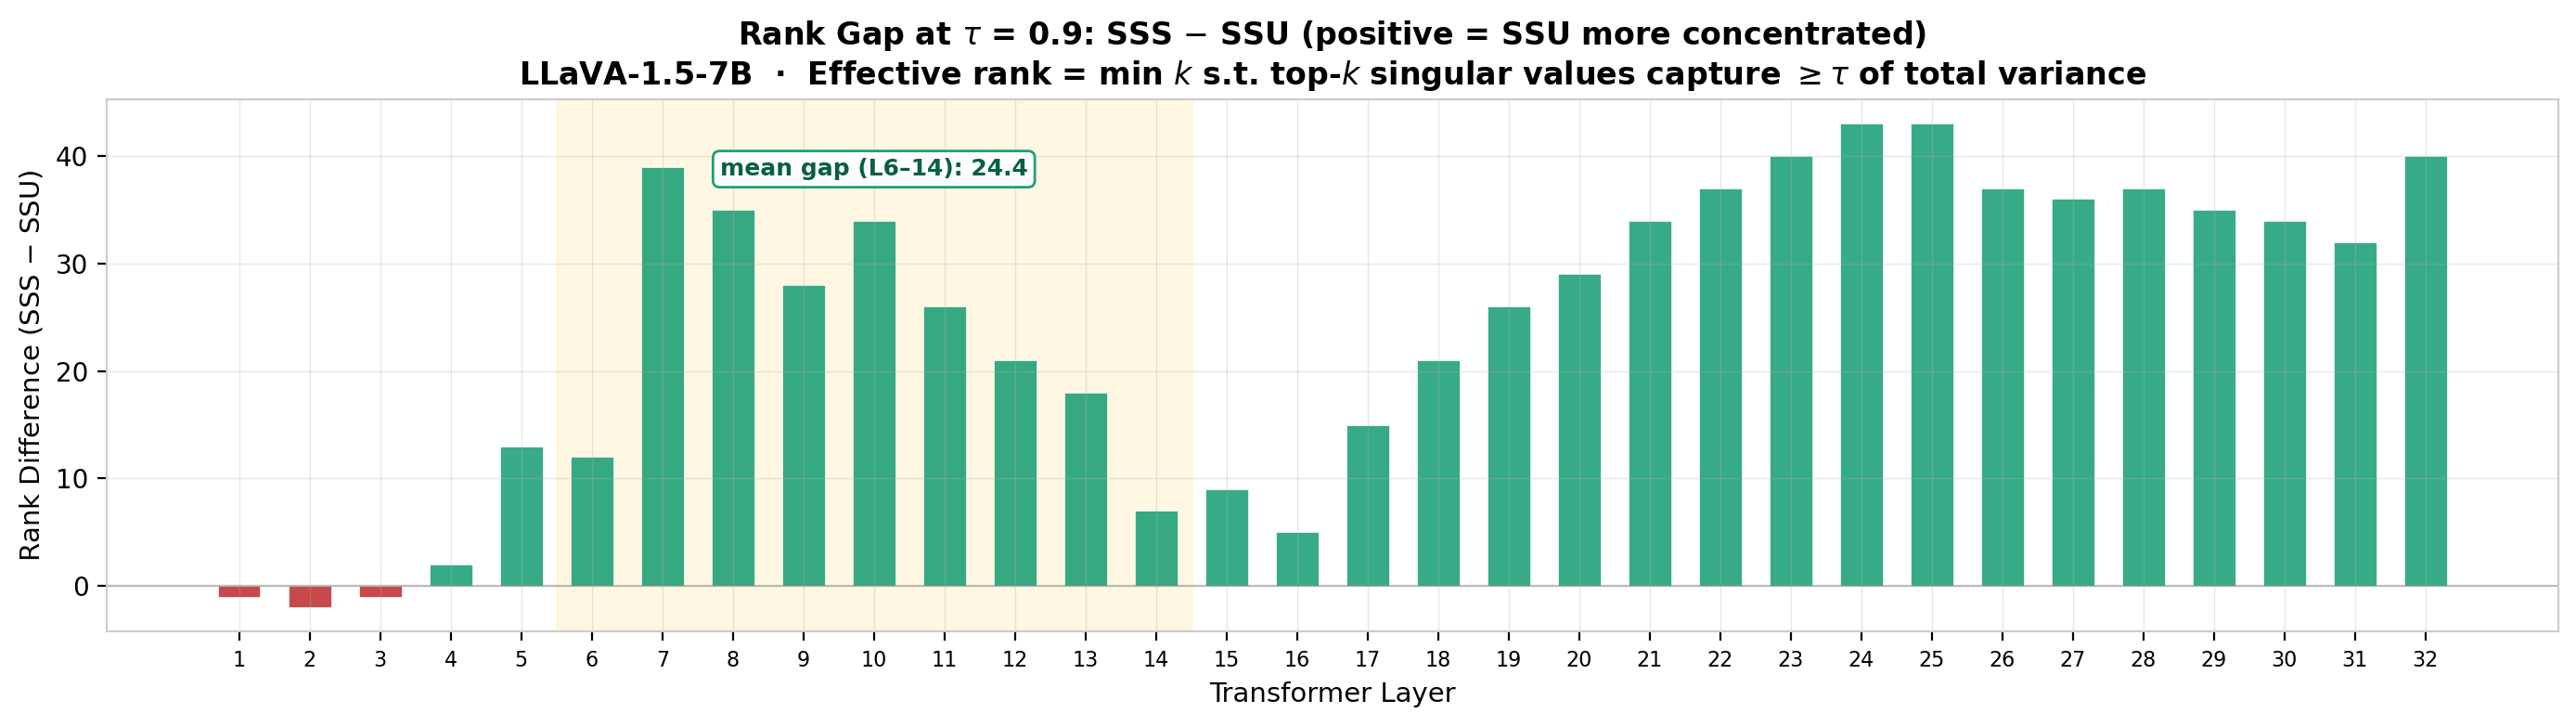
\includegraphics[width=\linewidth]{rank_gap}
    \caption{Rank difference (\sss{} $-$ \ssu{}) at $\tau{=}0.9$ across layers.
             Three-phase dynamics are clearly visible.}
    \label{fig:rank_gap}
  \end{subfigure}
  \par\bigskip
  \begin{subfigure}[b]{0.48\linewidth}
    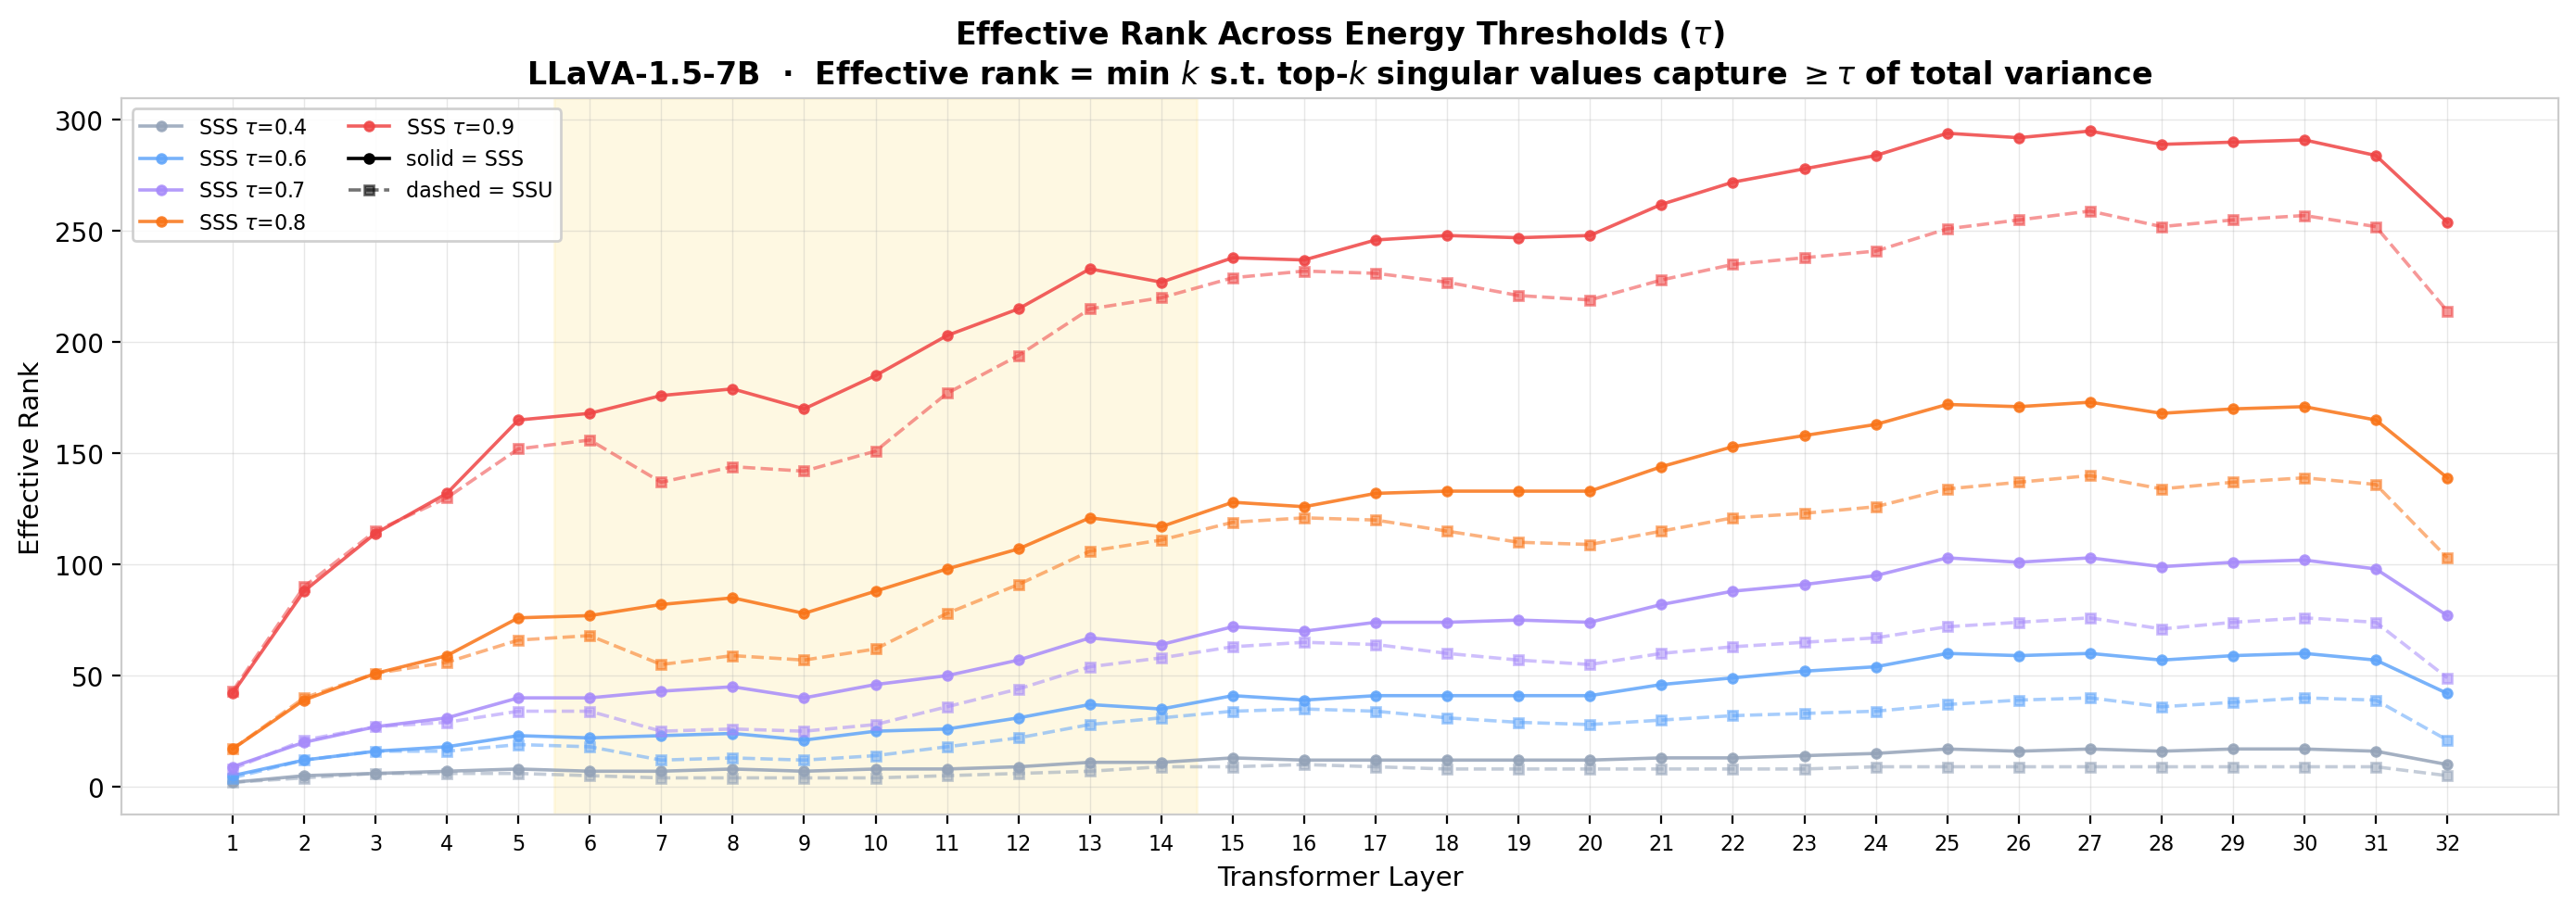
\includegraphics[width=\linewidth]{multi_threshold}
    \caption{Effective rank across multiple thresholds ($\tau{=}0.4$--$0.9$).
             Solid lines: \sss{}; dashed: \ssu{}.  The gap is consistent.}
    \label{fig:multi_threshold}
  \end{subfigure}
  \hfill
  \begin{subfigure}[b]{0.48\linewidth}
    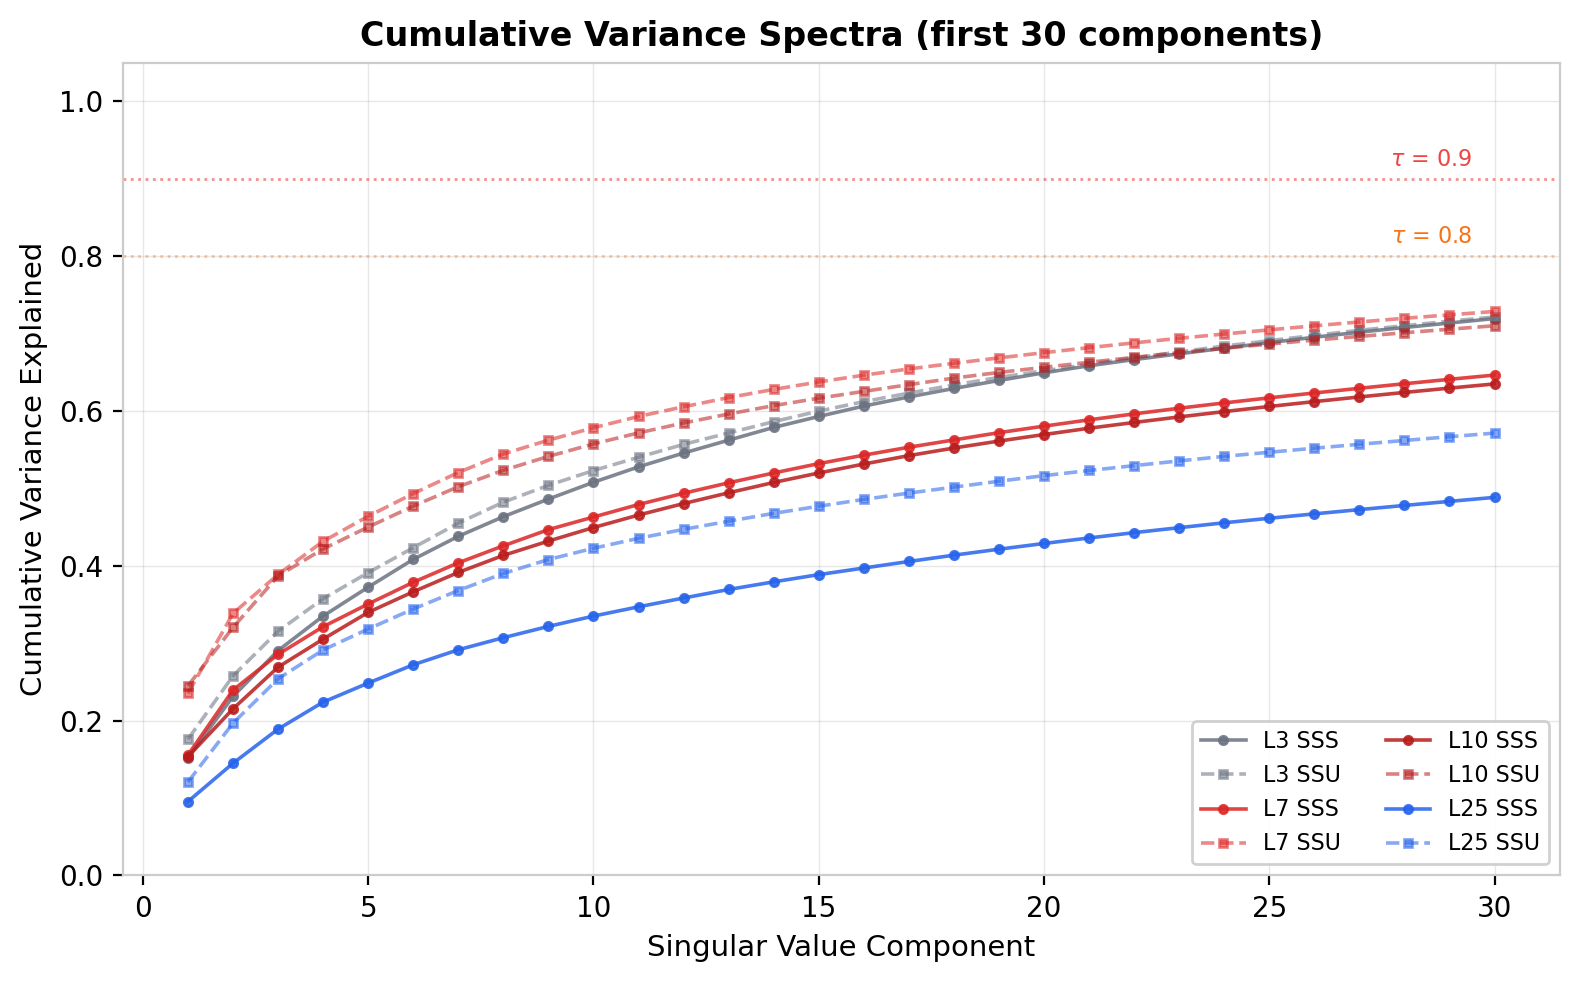
\includegraphics[width=\linewidth]{cumulative_variance_spectra}
    \caption{Cumulative variance explained by first 30 singular value components
             at representative layers (L3, L7, L10, L25).}
    \label{fig:cumulative_variance}
  \end{subfigure}
  \caption{Experiment A: Effective rank analysis.  \ssu{} modality shifts are
           consistently more concentrated than \sss{} in safety-critical layers.}
  \label{fig:effective_rank}
\end{figure}

\subsection{Experiment B: Safety Subspace Decomposition}
\label{sec:exp_b}

We decompose the safety subspace into its principal components via SVD and
analyze how the \ssu--\sss{} distortion is distributed across these dimensions.

\paragraph{Divergence from ShiftDC direction.}
The cosine similarity between the dominant SVD component $\mathbf{v}_1^l$ and
the ShiftDC direction $s^l$ is near-perfect in early layers ($|\cos| \approx 0.99$
at layer~1) but decays sharply through the safety-critical region ($|\cos| \approx
0.77$ at layers 7--8) and becomes nearly orthogonal by layer~17+
($|\cos| < 0.19$; Figure~\ref{fig:dom_vs_method2}).  This progressive divergence
indicates that the difference-in-means direction increasingly captures a
\emph{blend} of safety dimensions rather than the true dominant axis.

\paragraph{Safety distortion is multi-dimensional.}
The dominant component (component~0) explains a mean of 67.0\% of the variance
in the safety-relevant activation differences but accounts for only ${\sim}5\%$
of the total \ssu--\sss{} projection difference in layers 6--14.  The remaining
difference is distributed across components 1--9+, with an average of 8.6 out
of 10 components showing statistically significant \ssu{} vs.\ \sss{} separation
($p < 0.05$).  This demonstrates that cross-modal safety distortion is
inherently multi-dimensional and cannot be fully captured---or corrected---by a
single direction.

\begin{figure}[t]
  \centering
  \begin{subfigure}[b]{0.48\linewidth}
    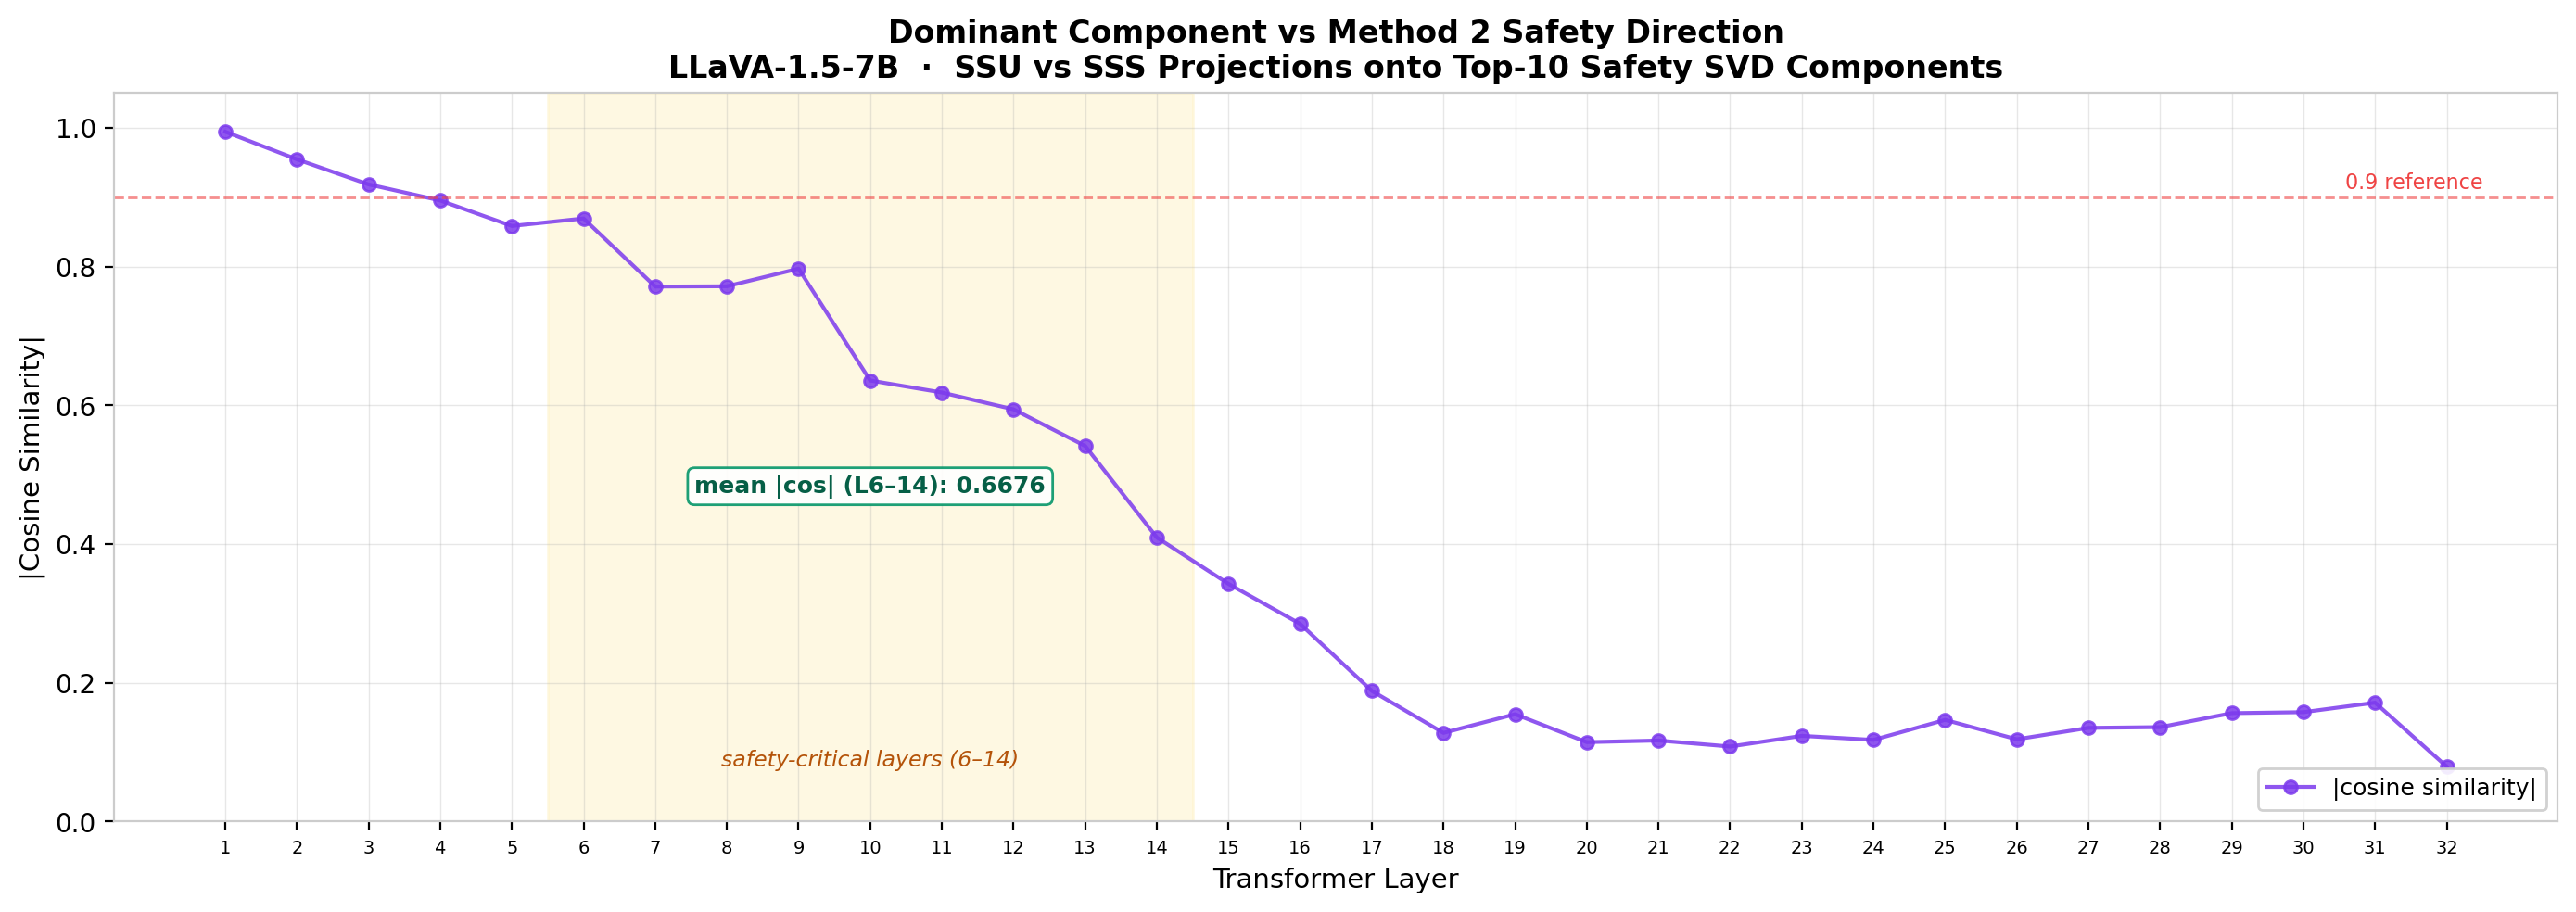
\includegraphics[width=\linewidth]{dominant_vs_method2_cosine}
    \caption{$|\cos(\mathbf{v}_1^l, s^l)|$ per layer.  Decays from ${\approx}1.0$
             in early layers to ${\approx}0.1$ in deep layers.}
    \label{fig:dom_vs_method2}
  \end{subfigure}
  \hfill
  \begin{subfigure}[b]{0.48\linewidth}
    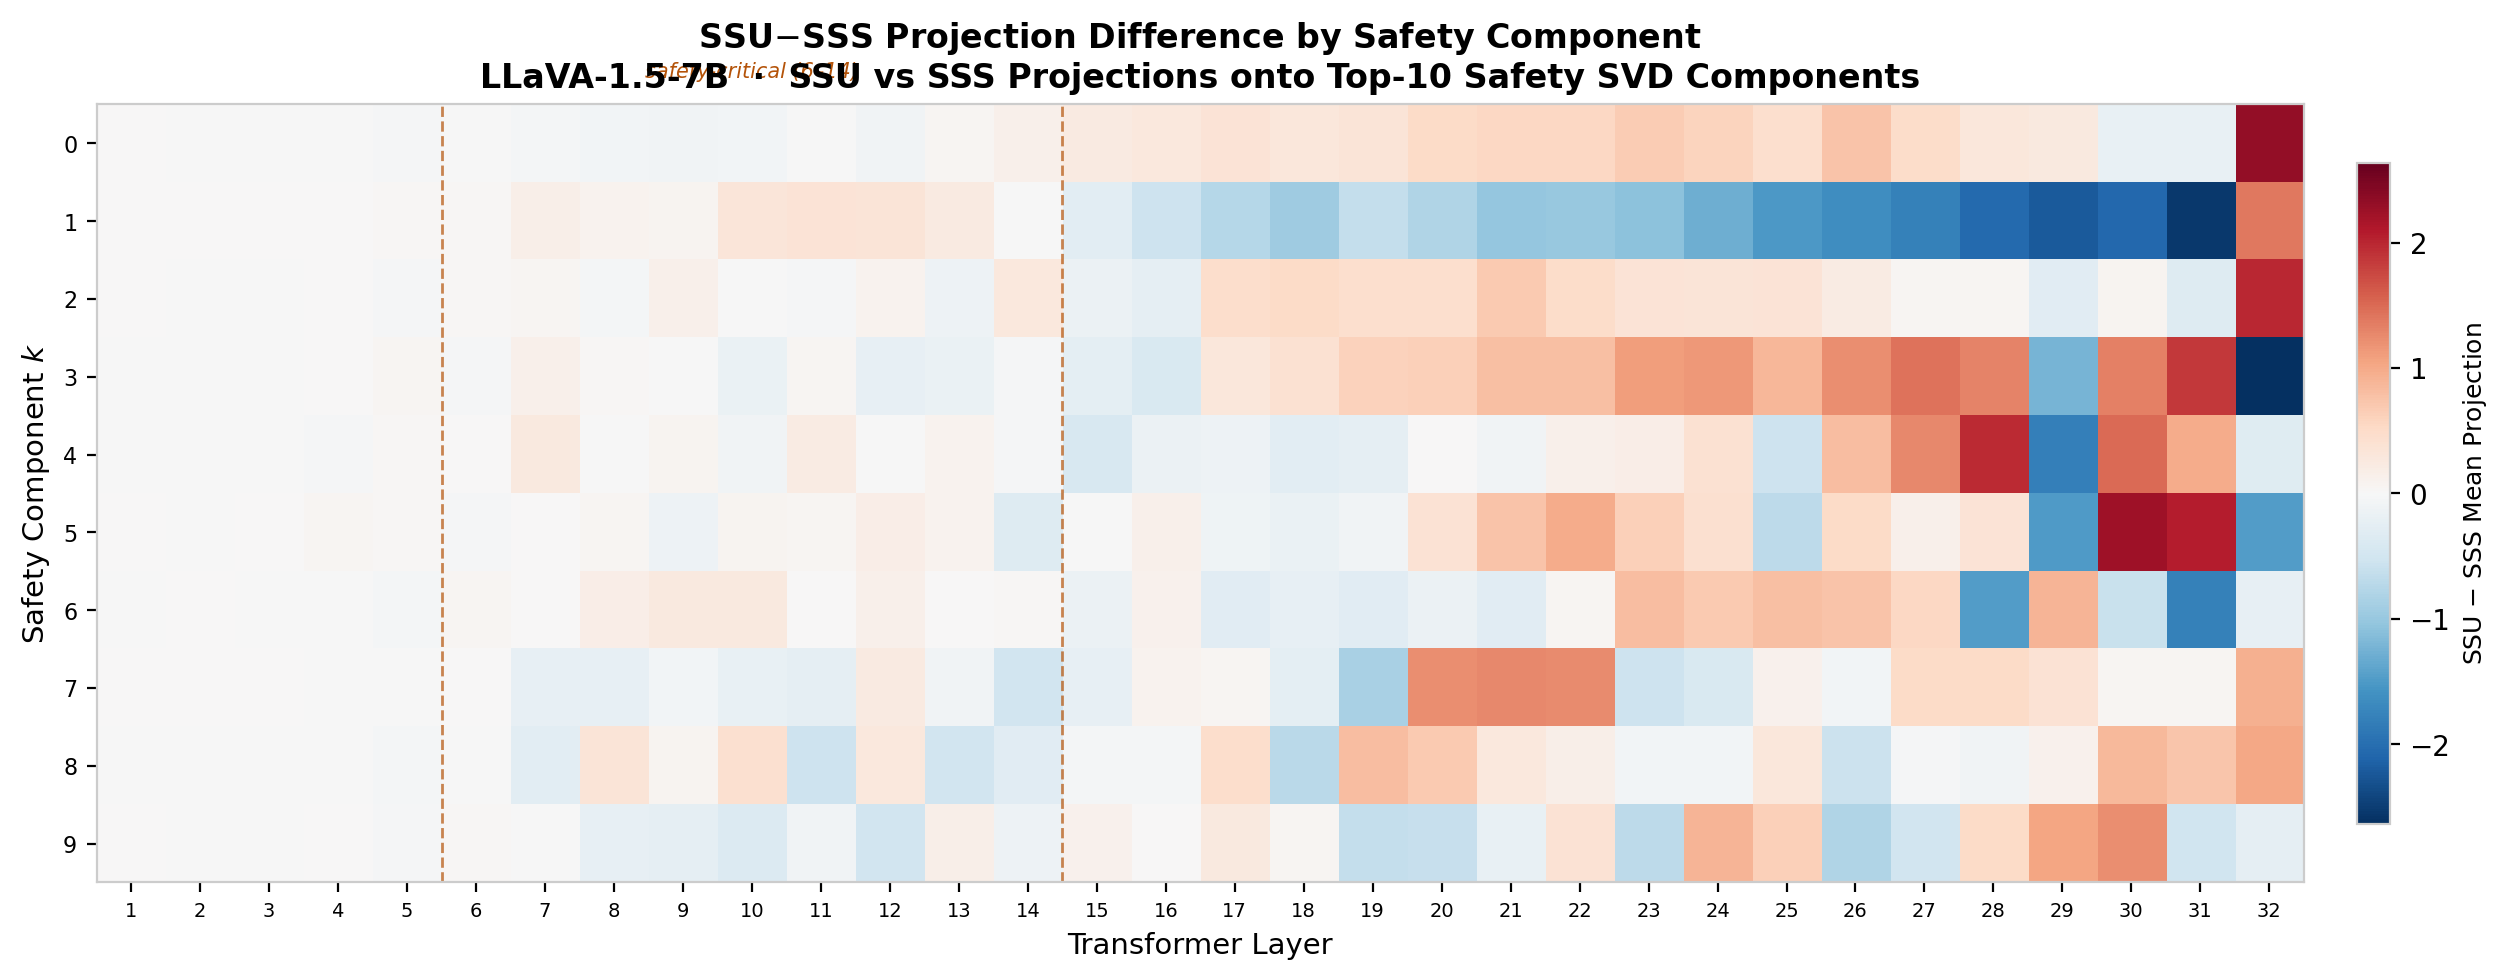
\includegraphics[width=\linewidth]{ssu_sss_projection_heatmap}
    \caption{Heatmap of \ssu{}$-$\sss{} mean projection difference across layers
             (x-axis) and safety components (y-axis).  Multi-dimensional
             distribution is evident.}
    \label{fig:heatmap}
  \end{subfigure}
  \par\bigskip
  \begin{subfigure}[b]{0.48\linewidth}
    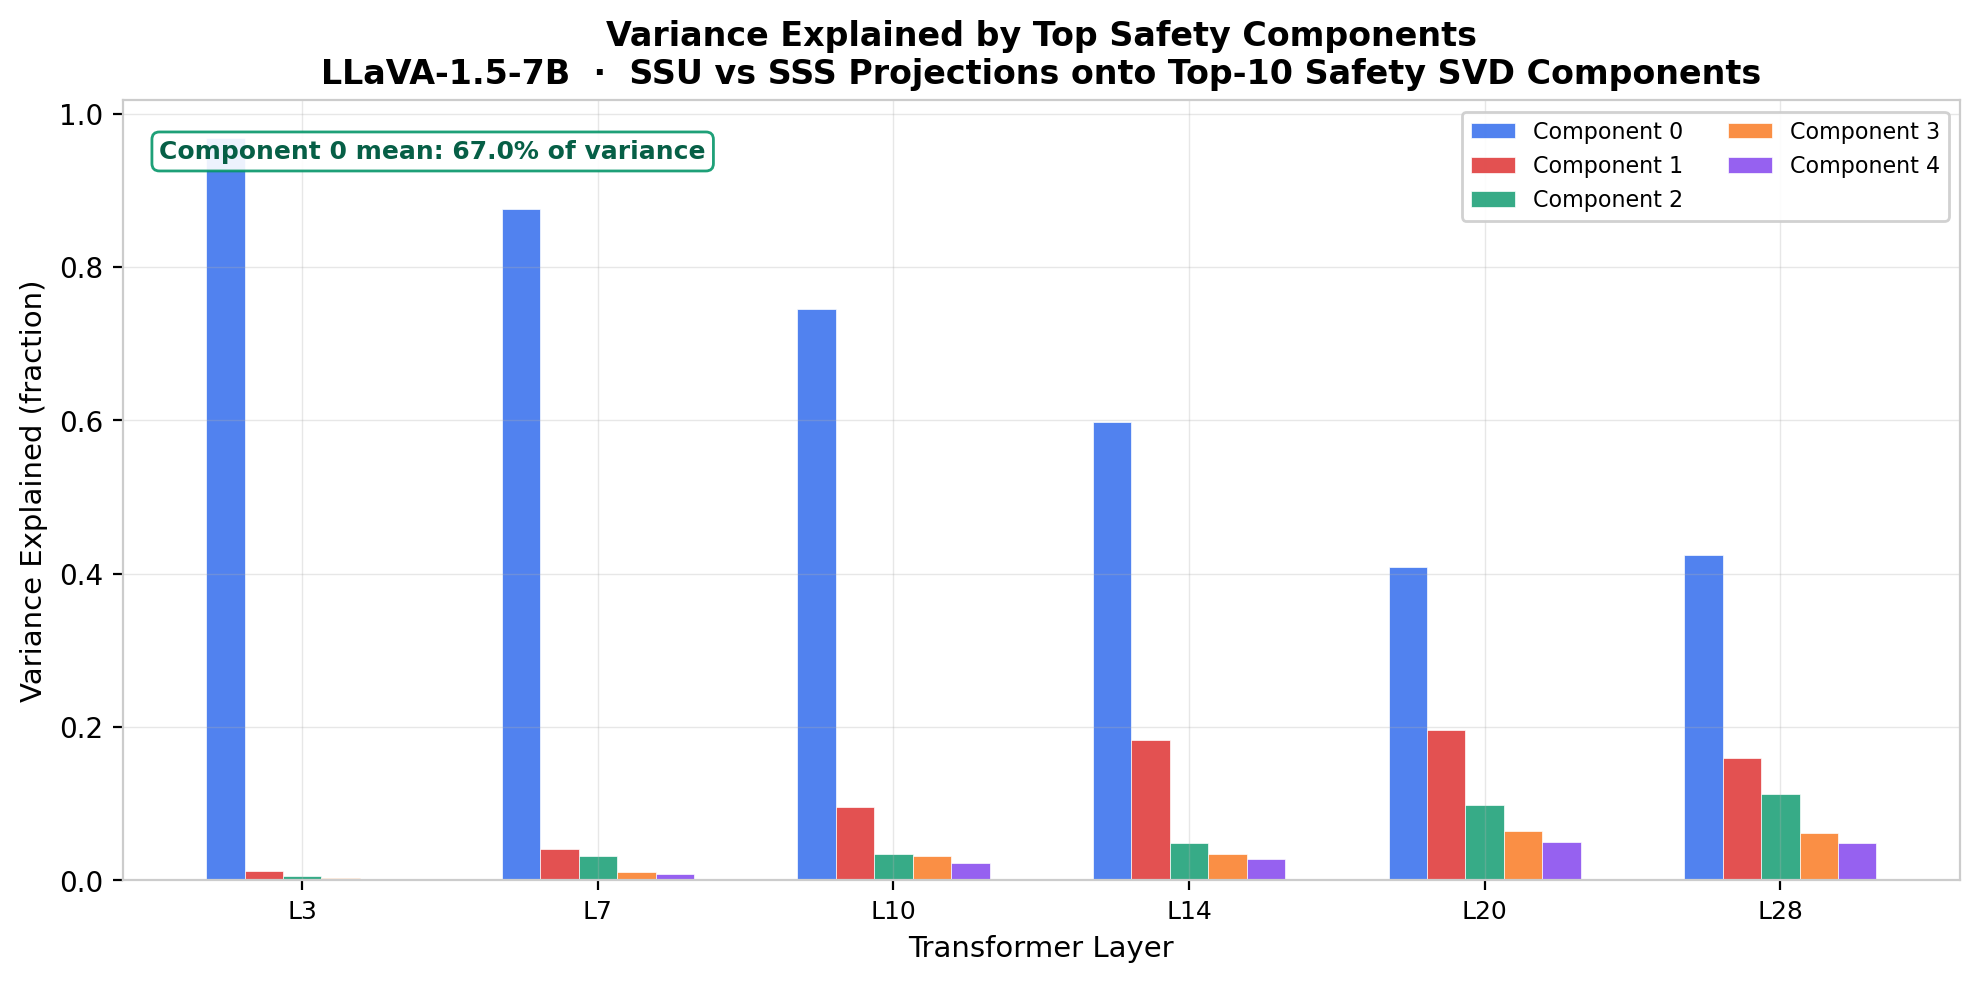
\includegraphics[width=\linewidth]{variance_explained}
    \caption{Variance explained by the top-5 safety components at representative
             layers (L3, L7, L10, L14, L20, L28).}
    \label{fig:variance_explained}
  \end{subfigure}
  \hfill
  \begin{subfigure}[b]{0.48\linewidth}
    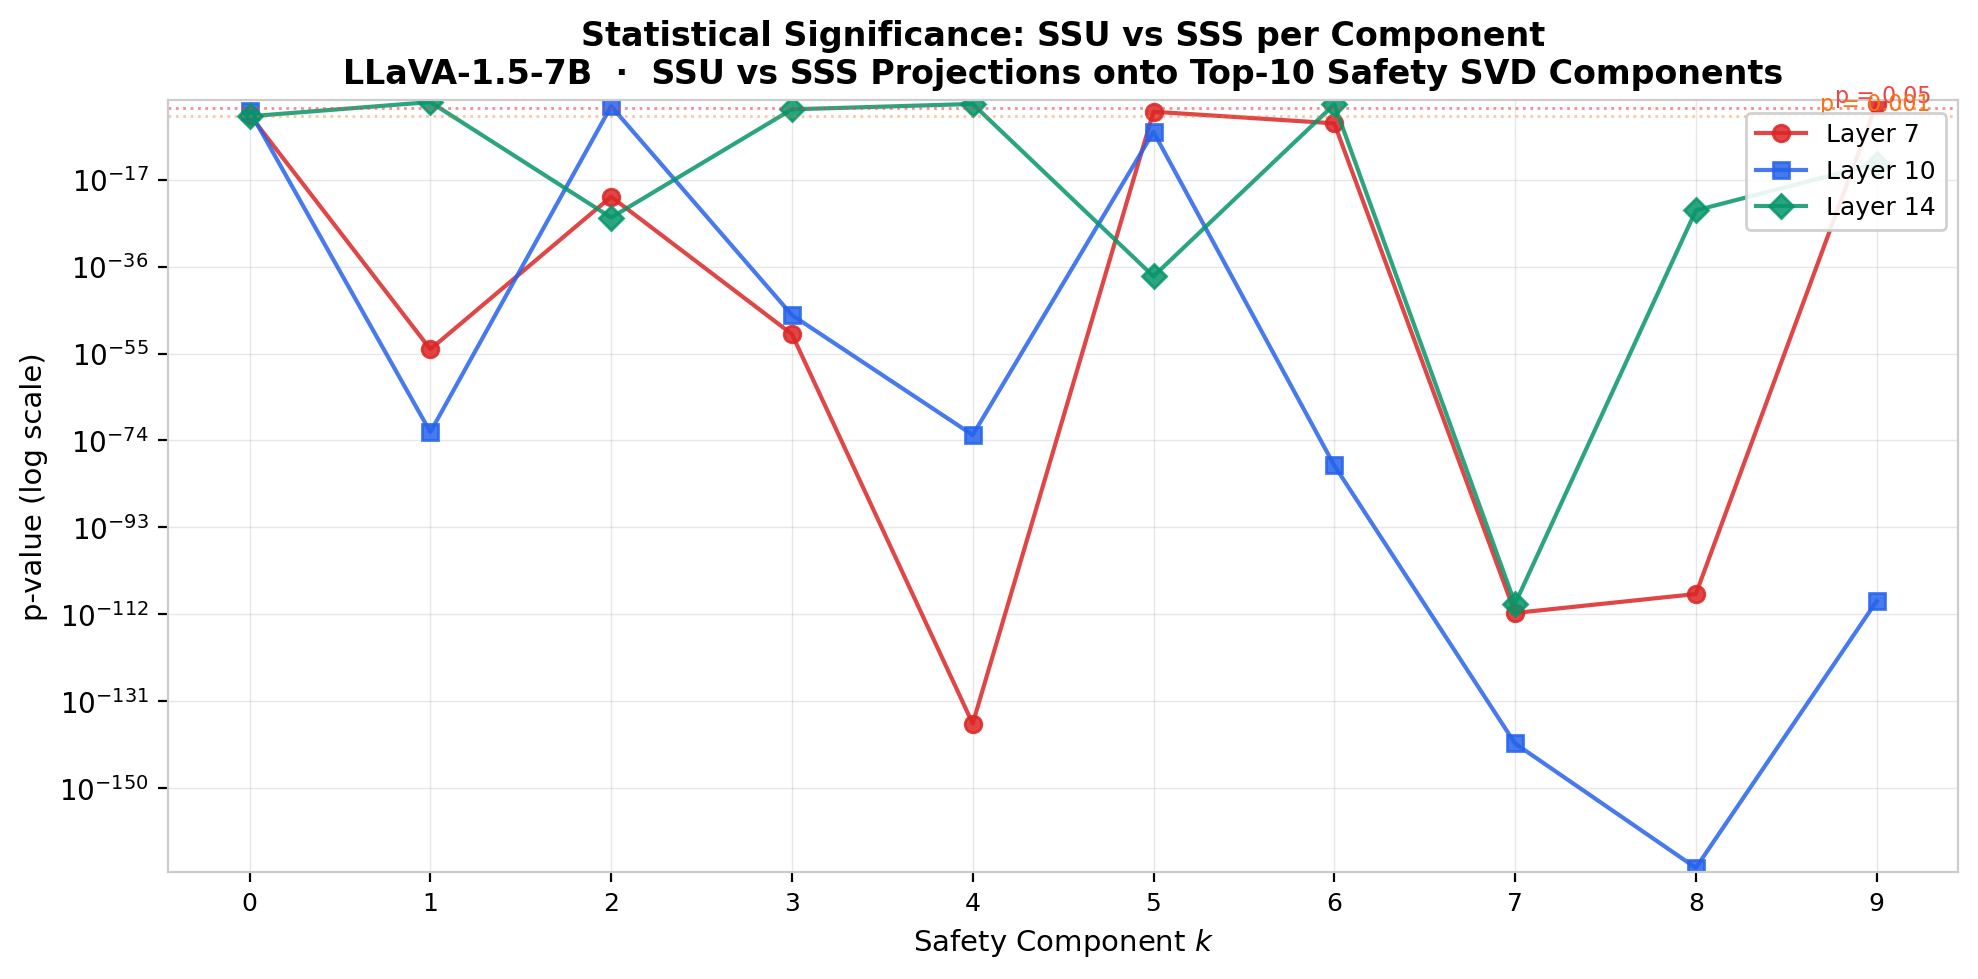
\includegraphics[width=\linewidth]{p_values_per_component}
    \caption{$-\log_{10}(p)$ of \ssu{} vs.\ \sss{} separation per component at
             layers~7, 10, and~14.  8+ of 10 components are significant.}
    \label{fig:pvalues_per_comp}
  \end{subfigure}
  \caption{Experiment B: Safety subspace decomposition.  The distortion is
           distributed across multiple orthogonal safety dimensions.}
  \label{fig:safety_decomp}
\end{figure}

\subsection{Experiment C: Subspace Overlap Between Integration and Safety Subspaces}
\label{sec:exp_c}

We extract the modality integration subspace for \sss{} and \ssu{} separately
via SVD of their respective modality shift matrices, and measure the geometric
overlap with the safety subspace using principal angles.

\paragraph{\sss{} integration overlaps more with safety.}
The \sss{} integration subspace has consistently higher overlap with the safety
subspace than the \ssu{} integration subspace across safety-critical layers
($L_{6\text{--}14}$ mean: \sss{} $= 0.228$, \ssu{} $= 0.182$, gap $=+0.047$;
Figure~\ref{fig:overlap}).  This is initially counterintuitive---if \ssu{} shifts
cause more safety distortion, why do they overlap \emph{less} with the safety
subspace?  The resolution lies in the distinction between \emph{breadth} and
\emph{precision} of safety-relevant displacement: \ssu{} shifts concentrate
their effect into a narrower portion of the safety subspace (lower effective rank),
while \sss{} shifts are more diffusely entangled with safety dimensions.

\paragraph{Distinct integration pathways.}
The direct overlap between \sss{} and \ssu{} integration subspaces is moderate
($L_{6\text{--}14}$ mean: 0.431), indicating the model routes visual information
through substantially different computational pathways depending on content.
This geometric distinction emerges precisely in the layers where safety
representations are active.

\paragraph{Robust to dimensionality.}
Sensitivity analysis over $k \in \{1,2,3,5,10,20\}$ shows the \sss{} $>$ \ssu{}
overlap pattern is stable across dimensionality choices (Figure~\ref{fig:sensitivity}).

\begin{figure}[t]
  \centering
  \begin{subfigure}[b]{0.48\linewidth}
    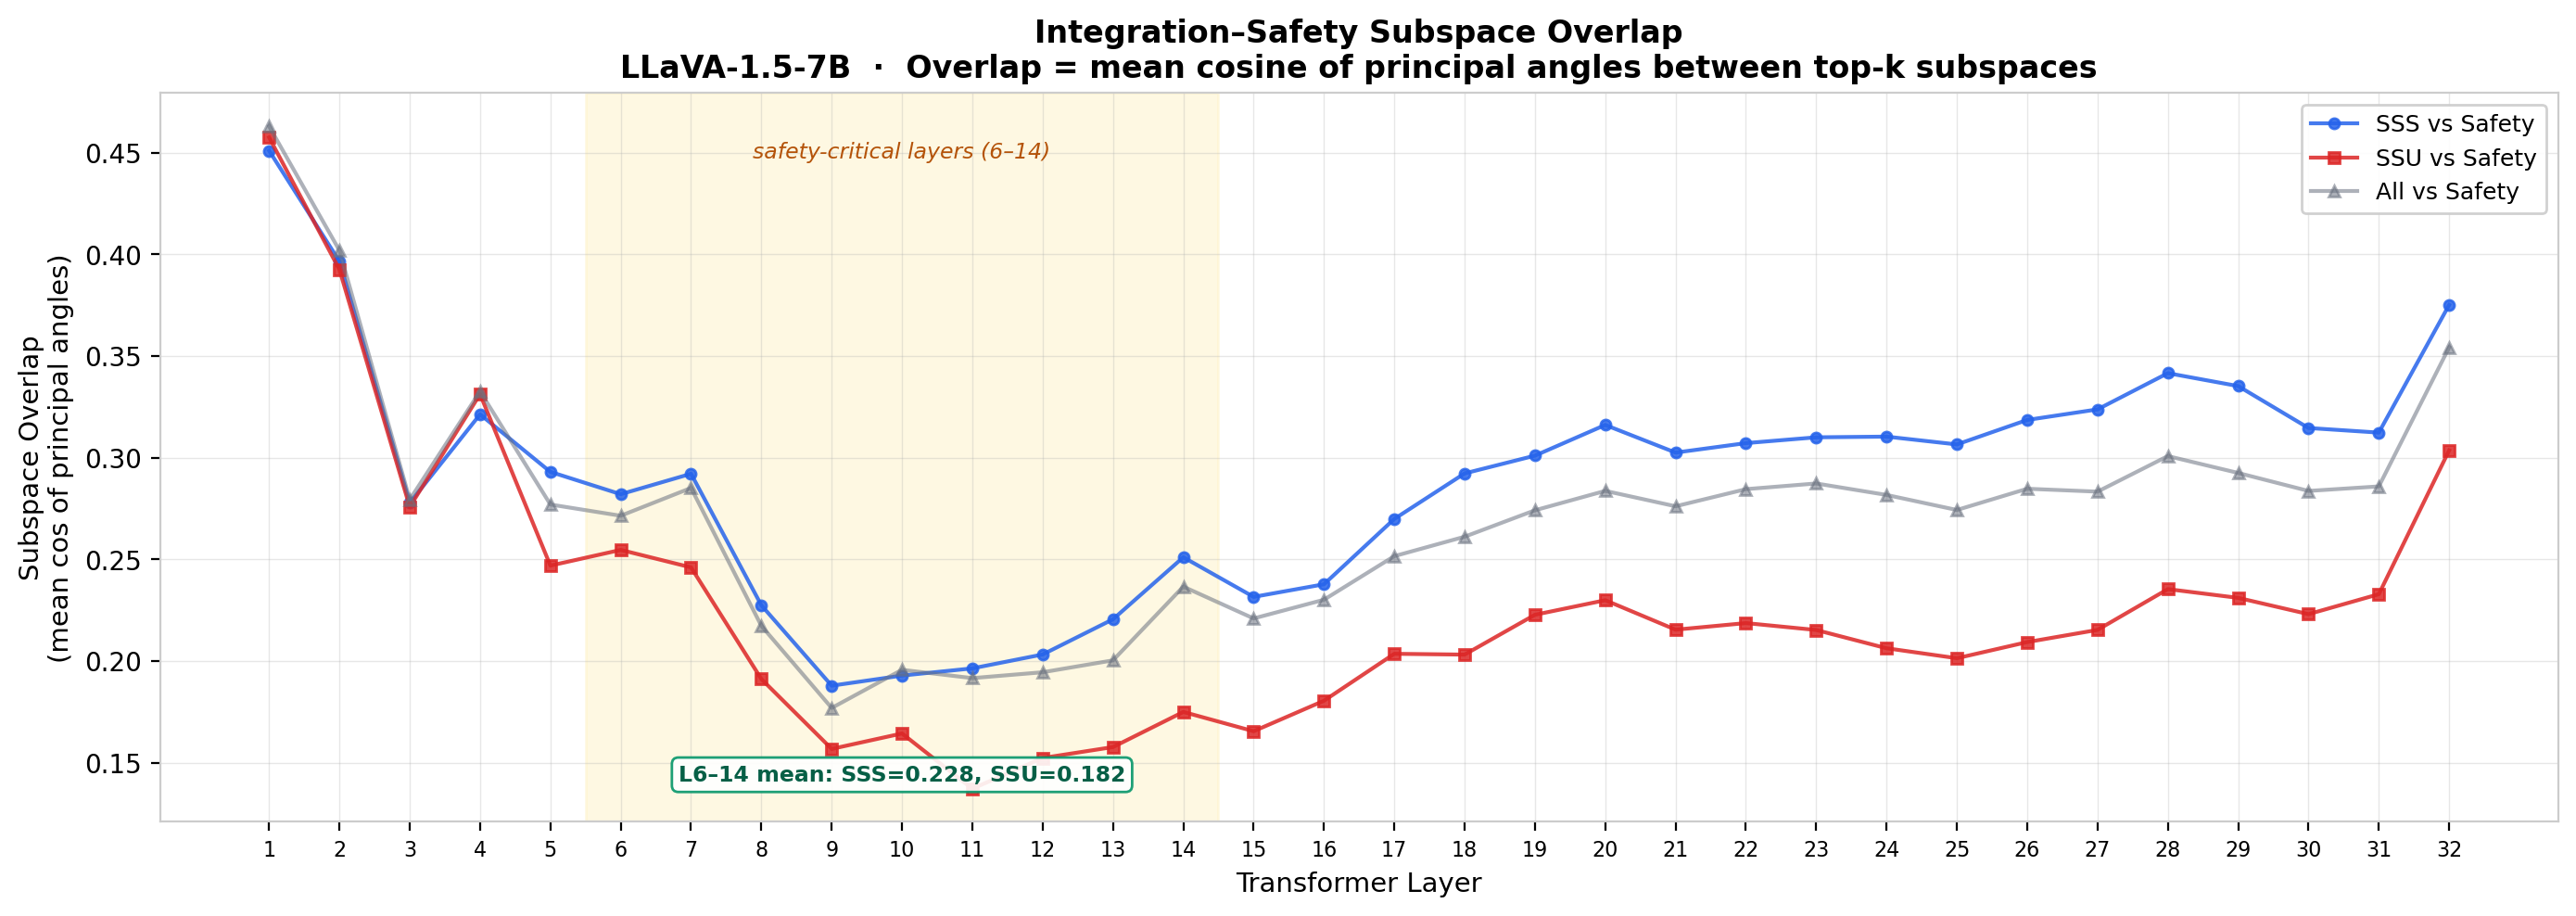
\includegraphics[width=\linewidth]{integration_safety_overlap}
    \caption{Per-layer subspace overlap between integration subspaces (\sss{},
             \ssu{}, combined) and the safety subspace.  \sss{} $>$ \ssu{}
             throughout safety-critical layers.}
    \label{fig:int_safety_overlap}
  \end{subfigure}
  \hfill
  \begin{subfigure}[b]{0.48\linewidth}
    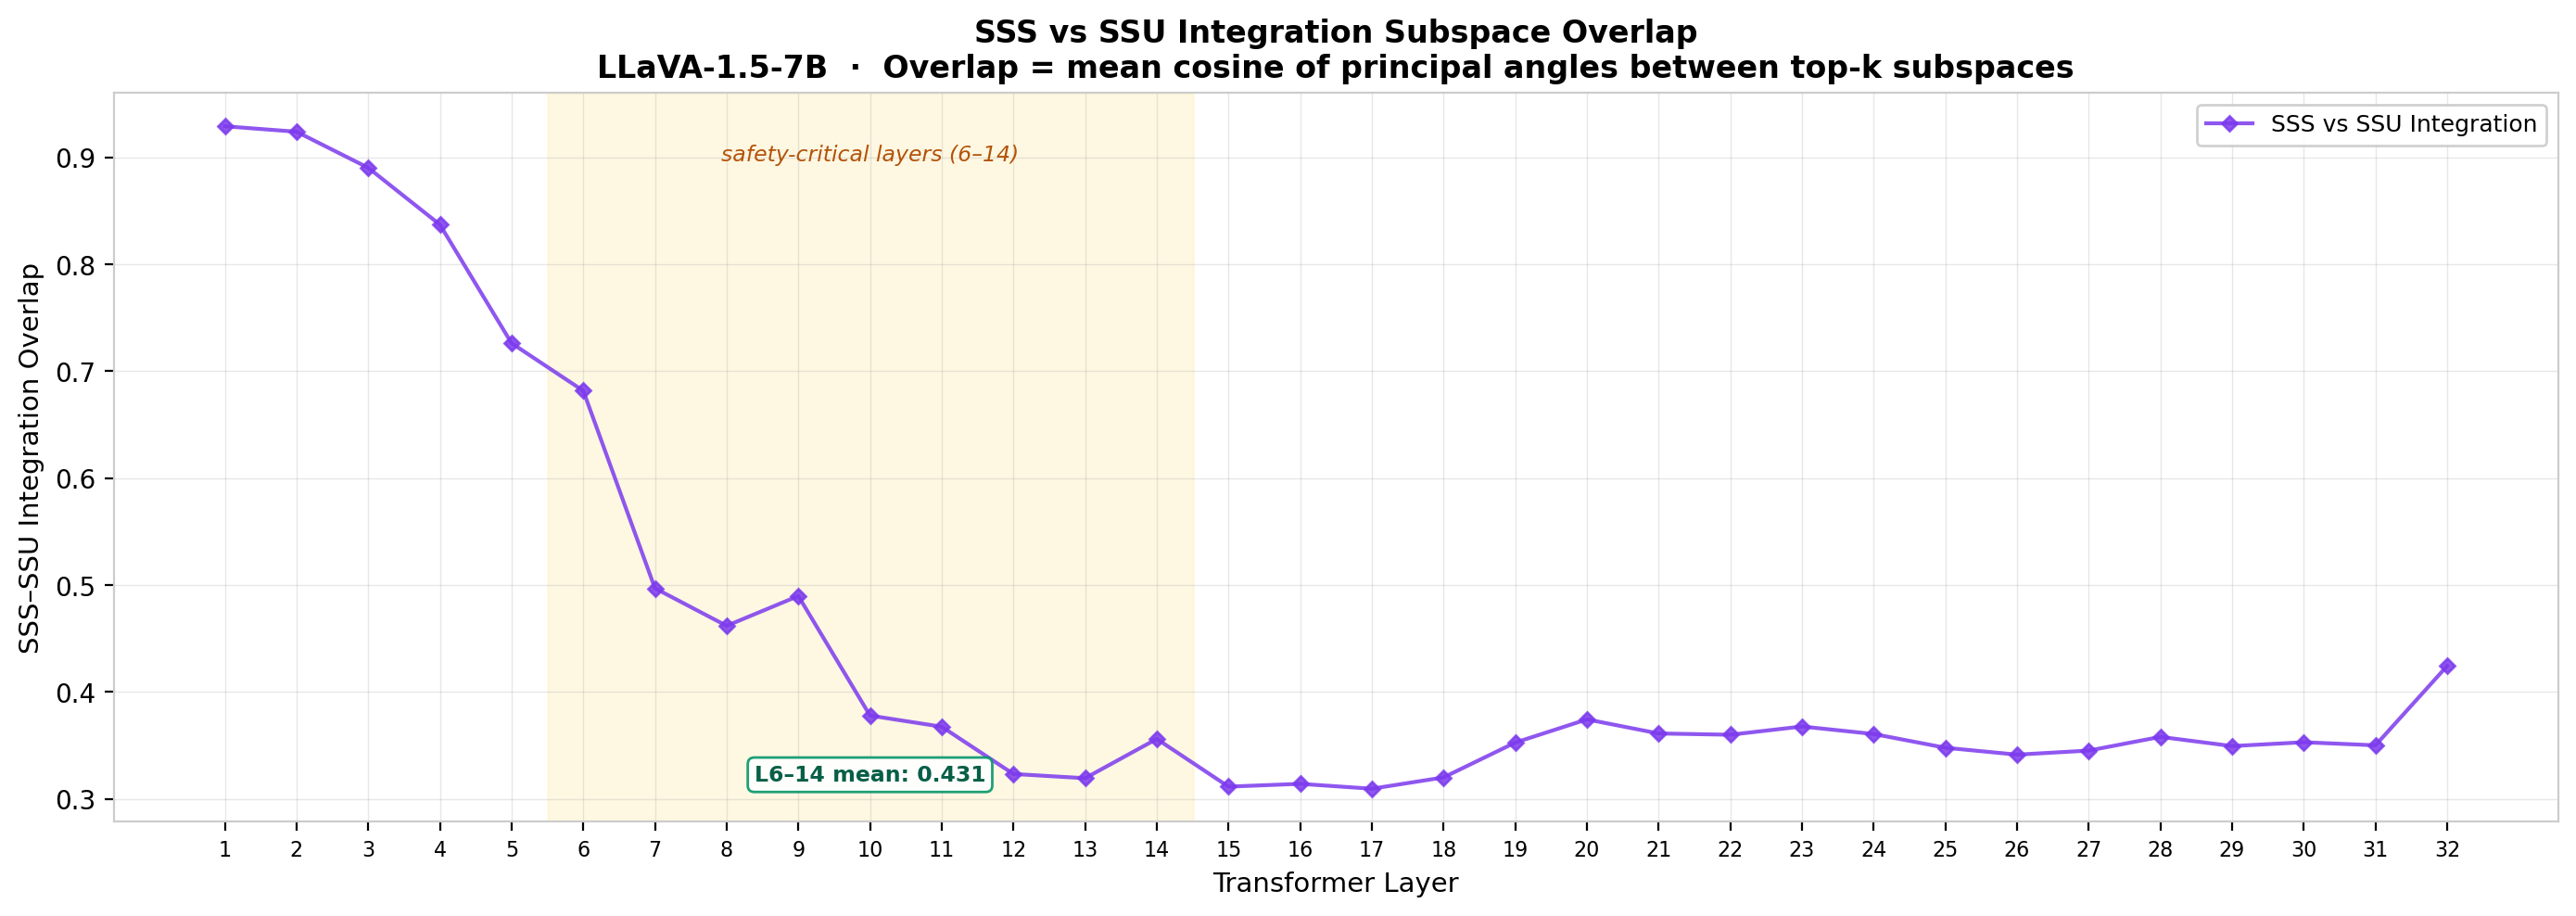
\includegraphics[width=\linewidth]{sss_ssu_integration_overlap}
    \caption{Per-layer overlap between \sss{} and \ssu{} integration subspaces.
             Moderate overlap (${\approx}0.43$) indicates geometrically distinct
             pathways.}
    \label{fig:sss_ssu_overlap}
  \end{subfigure}
  \par\bigskip
  \begin{subfigure}[b]{0.48\linewidth}
    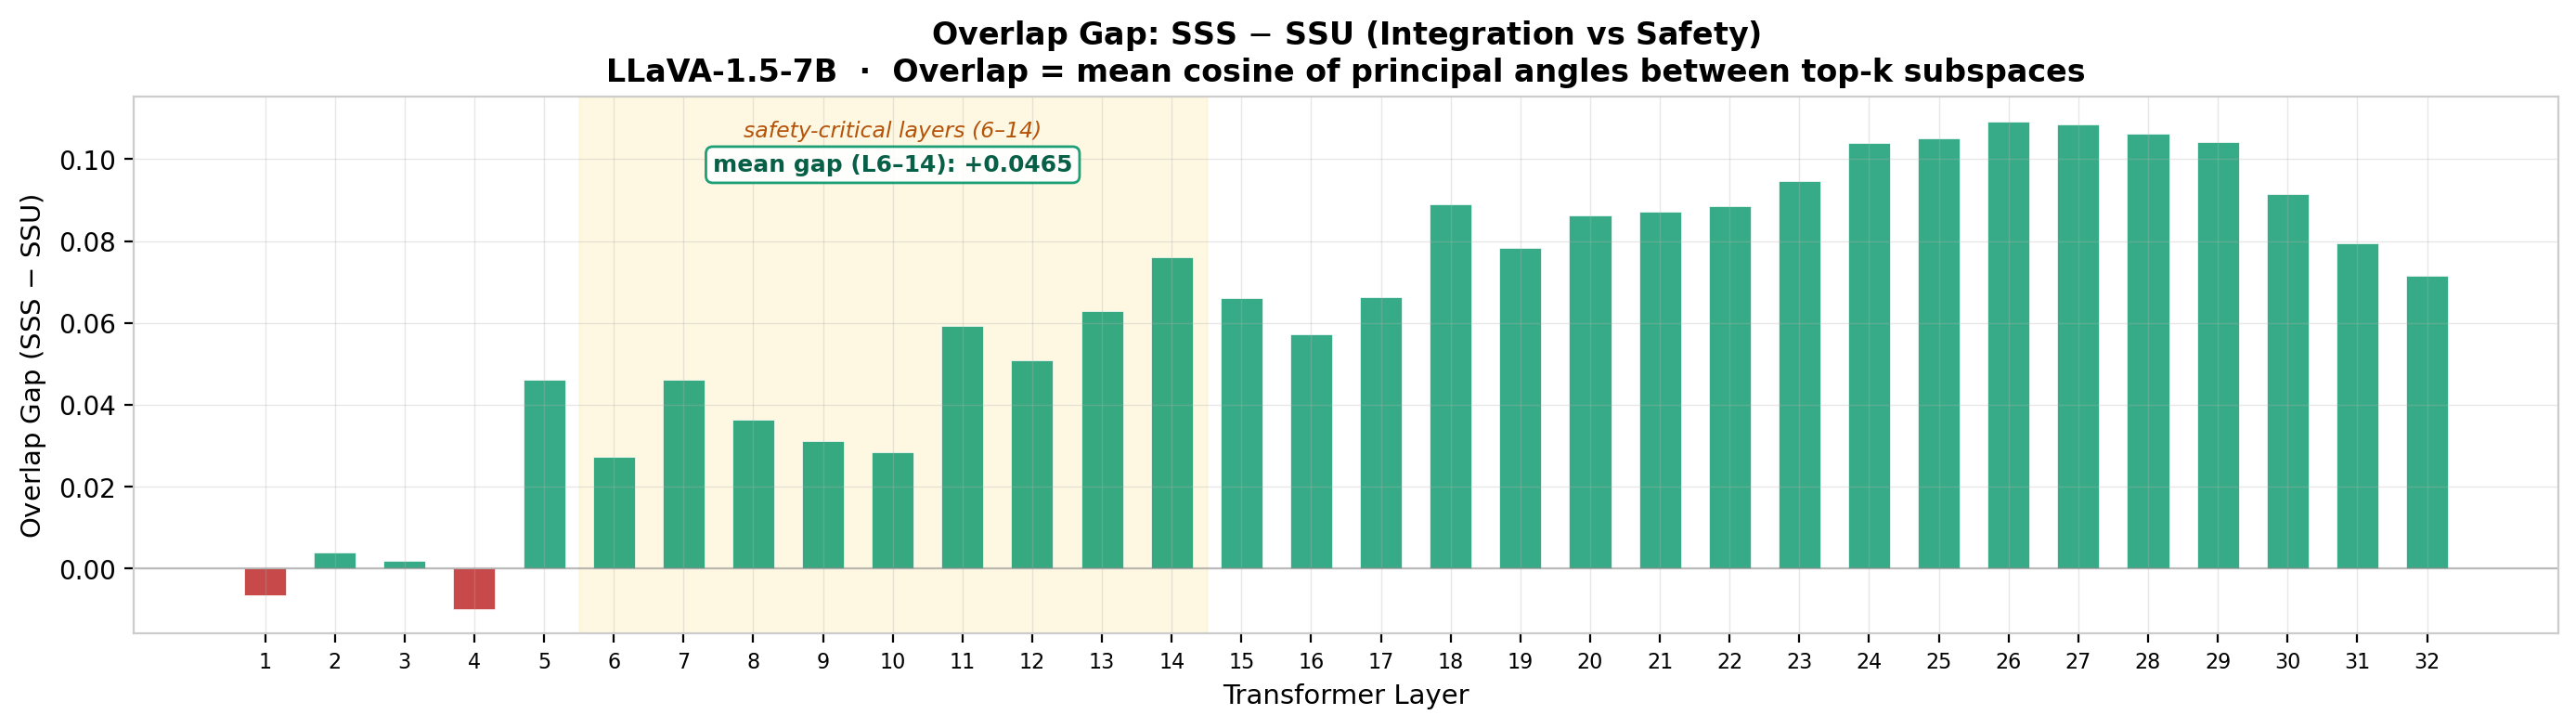
\includegraphics[width=\linewidth]{overlap_gap}
    \caption{Per-layer overlap gap (\sss{}$-$\ssu{}) for integration-vs-safety
             overlap.  Positive across all safety-critical layers.}
    \label{fig:overlap_gap}
  \end{subfigure}
  \hfill
  \begin{subfigure}[b]{0.48\linewidth}
    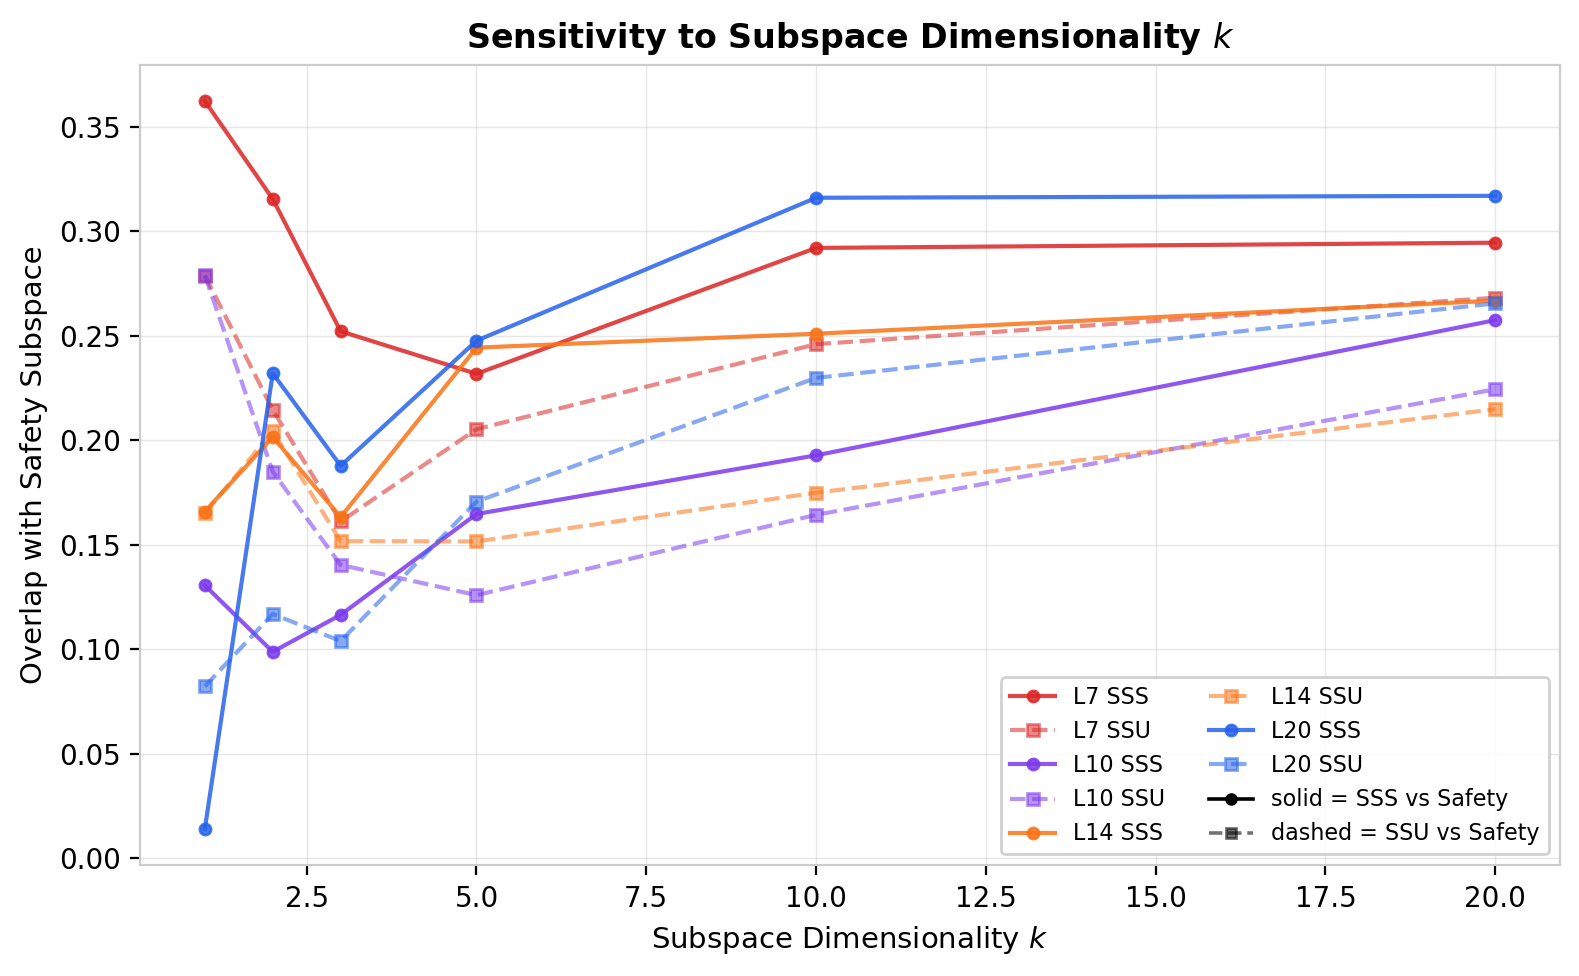
\includegraphics[width=\linewidth]{sensitivity_dimensionality}
    \caption{Sensitivity of overlap to $k$ at representative layers.  The
             \sss{} $>$ \ssu{} pattern is stable across dimensionality choices.}
    \label{fig:sensitivity}
  \end{subfigure}
  \caption{Experiment C: Subspace overlap analysis.  \sss{} and \ssu{} examples
           are processed through geometrically distinct modality integration
           pathways.}
  \label{fig:overlap}
\end{figure}

% ============================================================
\section{Discussion}
\label{sec:discussion}

\subsection{A Unified Geometric Picture of Cross-Modal Safety Distortion}

Our experiments paint a coherent geometric picture of why Safe+Safe$\to$Unsafe
failures occur:

\begin{enumerate}
  \item \textbf{Pre-existing vulnerability.}  \ssu{} text-only inputs are
        positioned closer to the unsafe region than \sss{} text-only inputs
        (\S\ref{sec:baseline}), even though both are individually safe.  This
        reflects subtle semantic features (\eg, references to chemicals, weapons,
        specific scenarios) that weakly activate safety-relevant representations.

  \item \textbf{Content-dependent routing.}  When images are introduced, the
        model processes \sss{} and \ssu{} inputs through geometrically distinct
        modality integration pathways (\S\ref{sec:exp_c}).  The \ssu{} pathway
        concentrates its effect along a narrower set of directions (lower
        effective rank, \S\ref{sec:exp_a}) that are more precisely aligned with
        the safety axis.

  \item \textbf{Multi-dimensional distortion.}  The resulting safety distortion
        is distributed across multiple orthogonal safety dimensions
        (\S\ref{sec:exp_b}), explaining why single-direction corrections achieve
        only partial effectiveness.

  \item \textbf{Active override of correct positioning.}  For the ${\sim}40\%$
        of \ssu{} examples whose text-only baselines are already correctly
        positioned on the safe side, the image integration process actively
        overrides correct safety assessments (\S\ref{sec:baseline}).
\end{enumerate}

\subsection{Implications for Correction Methods}

\paragraph{Single-direction methods are fundamentally limited.}
ShiftDC removes the projection of the modality shift onto a single safety
direction $s^l$.  Our Experiment~B shows that this direction captures only
${\sim}5\%$ of the total \ssu--\sss{} projection difference in safety-critical
layers, and that the direction itself diverges from the true dominant safety
component in deeper layers.  Any single-direction method will leave the remaining
${\sim}95\%$ of multi-dimensional distortion uncorrected.

\paragraph{Subspace-level correction is necessary.}
A natural extension is to project out the top-$K$ safety components from the
modality shift, rather than just the top-1.  Our Experiment~B provides the
requisite bases for such a correction, and the variance explained analysis gives
guidance on choosing~$K$.

\paragraph{Pathway-specific intervention is possible.}
The distinct geometric signatures of \sss{} and \ssu{} integration pathways
suggest that one could classify which pathway a given input is being processed
through and apply correction only when \ssu-like integration patterns are
detected, analogous to CAST's conditional activation steering~\citep{bai2024cast}
but operating on multi-dimensional subspaces.

\subsection{Limitations}

Our analysis is conducted on a single model (LLaVA-1.5-7B) and a single
benchmark (HoliSafe-Bench).  The most significant methodological limitation is
that the safety direction extraction via difference-in-means---inherited from
ShiftDC and used throughout our experiments---inherits confounding issues where
the safe and unsafe reference datasets differ in topic and vocabulary, not just
safety.  While our SVD decomposition in Experiment~B partially mitigates this by
extracting multiple components from the reference data, a cleaner extraction using
matched contrastive pairs (as in CAST~\citep{bai2024cast}) would strengthen all
downstream analyses; we describe this upgrade as the first priority in
\S\ref{sec:future_direction}.  Additionally, our experiments are purely
diagnostic; we have not yet implemented or evaluated the subspace-level correction
methods our findings motivate.

% ============================================================
\section{Future Work}
\label{sec:future}

\subsection{Principled Safety Direction Extraction}
\label{sec:future_direction}

The most immediate methodological improvement is to replace the
difference-in-means safety direction (inherited from ShiftDC) with a more
principled extraction based on contrastive pairs and PCA, following the approach
of CAST~\citep{bai2024cast}.  The current safety direction
$s^l = \operatorname{ActMean}^l(D_{\mathrm{safe}}^{\mathrm{tt}}) -
\operatorname{ActMean}^l(D_{\mathrm{unsafe}}^{\mathrm{tt}})$ suffers from a
well-known confounding problem: the safe and unsafe reference datasets differ not
only in safety but also in topic, vocabulary, and semantic domain.  The extracted
direction therefore captures aggregate distributional differences rather than a
pure safety signal.

\subsubsection*{Extraction Technique: CAST Condition Vectors}

CAST defines two types of steering vectors: \emph{behavior vectors} (capturing
refusal vs.\ compliance responses) and \emph{condition vectors} (capturing
whether an input is harmful vs.\ harmless).  The safety direction we require maps
to CAST's \textbf{condition vector}---a direction that captures
``this input is unsafe'' vs.\ ``this input is safe'' in activation space.  This
distinction determines the extraction procedure: behavior vectors average hidden
states only over response suffix tokens, while condition vectors use the full
prompt representation.

The extraction applies PCA to a matrix of mean-centered contrastive activations
to find the direction of maximum variance:
\begin{equation}
  \mathbf{s}^l_{\mathrm{PCA}} = \operatorname{PCA}_1\!\left(
    \begin{bmatrix}
      h_1^+ - \mu_l \\ h_1^- - \mu_l \\ \vdots \\ h_n^+ - \mu_l \\ h_n^- - \mu_l
    \end{bmatrix}
  \right),
  \quad
  \mu_l = \frac{H_l^+ + H_l^-}{2},
  \label{eq:cast_pca}
\end{equation}
where $H_l^+$ and $H_l^-$ are the hidden states for harmful ($D^+$) and harmless
($D^-$) examples at layer~$l$, and the first principal component becomes the
safety direction for that layer.  The mean-centering step ensures the principal
component captures the safe/unsafe distinction rather than any overall offset.
Rows are interleaved (alternating positive and negative examples) before PCA,
following the CAST implementation.

\subsubsection*{Contrastive Dataset Construction}

CAST uses two published, peer-reviewed datasets: \textbf{Sorry-Bench}~\citep{xie2024sorrybench}
as the source of harmful prompts ($D^+$) and \textbf{Alpaca}~\citep{taori2023alpaca}
as the source of harmless prompts ($D^-$).  Both provide broad coverage---Sorry-Bench
spans diverse safety-relevant categories, and Alpaca provides general-purpose
instructions that are unambiguously benign.  Equal-sized subsets should be sampled
from each to avoid class imbalance artifacts in the PCA.  Using these published
datasets rather than custom examples has two advantages: (1)~reproducibility---any
reviewer can verify the construction; and (2)~the datasets have been validated
through peer review, reducing systematic biases in prompt construction.

\subsubsection*{Token Position and Modality Considerations}

While CAST's default condition vector extraction averages hidden states over all
tokens, our downstream analyses (modality shift projections, baseline positioning,
safety subspace decomposition) all operate on \textbf{last-token hidden states}.
For consistency, the contrastive extraction should similarly use last-token
activations.  CAST's own appendix notes that last-token extraction may be more
informative for longer prompts, supporting this choice.

Critically, the contrastive extraction should remain entirely in
\textbf{text-only space} (no images), matching our current reference data
pipeline.  This ensures the extracted safety direction reflects the LLM
backbone's native safety representations without any vision-modality
interference---exactly the reference frame needed for measuring how image
integration distorts those representations.

\subsubsection*{Implementation Steps}

The concrete steps to implement this upgrade are:

\begin{enumerate}
  \item \textbf{Prepare contrastive data.}  Sample $n$ harmful prompts from
        Sorry-Bench and $n$ harmless prompts from Alpaca (\eg, $n{=}200$).
        Format each as a text-only input to LLaVA-1.5-7B (no image; prompt only,
        appended with the assistant token prefix).

  \item \textbf{Collect hidden states.}  Run forward passes for all $2n$ prompts
        in text-only mode.  At each layer~$l$, extract the last-token hidden
        state $h_i^l \in \mathbb{R}^d$.

  \item \textbf{Compute PCA safety direction per layer.}  For each layer~$l$:
        compute the global mean $\mu_l = \frac{1}{2n}\sum_i h_i^l$; mean-center
        all activations; stack into a matrix with interleaved rows
        $[\tilde{h}_1^+, \tilde{h}_1^-, \ldots] \in \mathbb{R}^{2n \times d}$;
        and extract the first principal component via SVD to obtain
        $\mathbf{s}^l_{\mathrm{PCA}}$.

  \item \textbf{Save per-sample activations.}  Unlike the current pipeline, save
        the individual reference activation vectors (not just the resulting
        direction) to enable downstream SVD decomposition in Experiment~B.  Save
        as \texttt{reference\_activation\_matrices.npz} with keys
        \texttt{safe\_layer\_\{l\}} and \texttt{unsafe\_layer\_\{l\}}.

  \item \textbf{Re-run all downstream experiments.}  The safety direction is
        upstream of the ShiftDC diagnostic, the sanity check, the centered
        projections, and the safety subspace decomposition (Experiment~B).  All
        must be re-run with the new direction.  Experiments A and C can
        optionally be re-run but are less sensitive to the safety direction choice.

  \item \textbf{Compare old vs.\ new directions.}  As a validation step, compute
        $|\cos(\mathbf{s}^l_{\mathrm{DIM}}, \mathbf{s}^l_{\mathrm{PCA}})|$ at
        each layer.  High similarity in early layers (where confounding is
        minimal) and divergence in deeper layers would confirm the upgrade matters
        most precisely where we need it most.
\end{enumerate}

We view this as the essential first step before pursuing the other directions
below, as a cleaner safety direction would either validate the robustness of our
current findings or reveal that certain patterns were artifacts of the confounded
extraction methodology.

\subsection{Near-Term Empirical Extensions}

\paragraph{Subgroup analysis of \ssu{} modality shift magnitudes.}
The centered baseline analysis (\S\ref{sec:baseline}) naturally partitions \ssu{}
samples into those that start on the safe side (${\sim}40\%$) and those that start
on the unsafe side (${\sim}60\%$).  Comparing the magnitude and geometric
properties of the modality shift between these two subgroups would further
disentangle the regression-to-mean and active distortion components.

\paragraph{Per-category analysis.}
HoliSafe-Bench spans multiple safety categories (violence, self-harm, illegal
activity, \etc).  Analyzing whether certain categories exhibit stronger distortion
or different geometric properties could reveal category-specific vulnerabilities.

\paragraph{Subspace-level correction implementation and evaluation.}
The most immediate practical direction is multi-dimensional ShiftDC: project out
the top-$K$ safety subspace components from the modality shift at inference time.
This method should be evaluated against ShiftDC, ECSO, and AdaShield on both
safety benchmarks (MM-SafetyBench, HoliSafe-Bench) and utility benchmarks (MME,
MM-Vet).

\paragraph{Conditional subspace correction.}
Leveraging the distinct integration pathway signatures from Experiment~C, one
could train a lightweight classifier on the modality shift vector to detect
\ssu-like integration patterns, then apply subspace-level correction only when
triggered.  This mirrors CAST's conditional steering but operates in the
integration subspace.

\subsection{Cross-Checkpoint Safety Subspace Analysis}

The Qwen-VL family provides a unique opportunity for cross-checkpoint analysis,
as all four checkpoints in the training pipeline are publicly available: (1)~Qwen-7B
(base LLM), (2)~Qwen-7B-Chat (LLM with RLHF/safety alignment), (3)~Qwen-VL
(VLM pretrained on base LLM), and (4)~Qwen-VL-Chat (VLM with instruction/safety
tuning).  Critically, the VLM is built on the \emph{base} LLM (stage~1), not the
chat-aligned version (stage~2), enabling several informative comparisons:

\begin{itemize}
  \item Comparing the safety subspaces of Qwen-7B-Chat (stage~2) and
        Qwen-VL-Chat (stage~4) would reveal whether VLM safety alignment
        rediscovers the same linear representations as text-only RLHF.
  \item Comparing Qwen-7B (stage~1) to Qwen-VL (stage~3) would isolate the
        effect of vision-language pretraining on safety-relevant geometry.
  \item Measuring whether SSU distortion severity correlates with the angular
        divergence between VLM-Chat and LLM-Chat safety directions would provide
        a quantitative link between architectural design and safety outcomes.
\end{itemize}

\subsection{Toward Robust Cross-Modal Safety}
\label{sec:future_robust}

Our geometric analysis suggests that robust cross-modal safety requires methods
aware of the multi-dimensional nature of safety representations and the
content-dependent nature of modality integration.  Promising directions include:

\begin{itemize}
  \item \textbf{Subspace-aware adversarial training:} Extending DPO or RLHF to
        explicitly regularize the safety subspace overlap between text-only and
        vision-language processing pathways.
  \item \textbf{Representation-level constraints during VLM pretraining:} Adding
        auxiliary losses that encourage the VLM to maintain the safety subspace
        geometry of the LLM backbone.
  \item \textbf{Cross-architecture validation:} Verifying whether the geometric
        patterns identified here generalize across Qwen2-VL, InternVL, and
        LLaMA-3.2-Vision.
\end{itemize}

% ============================================================
\section{Conclusion}
\label{sec:conclusion}

We have presented a systematic geometric analysis of cross-modal safety distortion
in Vision-Language Models, moving beyond single-direction analysis to reveal the
multi-dimensional subspace structure of the phenomenon.  Our experiments on
LLaVA-1.5-7B using HoliSafe-Bench establish that safety distortion from modality
integration is distributed across multiple orthogonal safety dimensions, that
\sss{} and \ssu{} examples are processed through geometrically distinct
integration pathways, and that the image integration process actively overrides
correct safety assessments for a substantial fraction of inputs.  These findings
explain the limitations of existing single-direction correction methods and
provide a principled foundation for the development of subspace-level
interventions that can more completely restore safety perception without
sacrificing multimodal understanding.

% ============================================================
\bibliographystyle{plainnat}
% NOTE: Create a file called "references.bib" in your Overleaf
% project (see template below) and uncomment the next line.
% \bibliography{references}

% ---- Inline bibliography (fallback if .bib is not set up) ----
\begin{thebibliography}{99}

\bibitem[Arditi et~al.(2024)]{arditi2024refusal}
Arditi, A., et~al.
\newblock Refusal in language models is mediated by a single direction.
\newblock \emph{NeurIPS 2024}.

\bibitem[Bai et~al.(2024)]{bai2024cast}
Bai, B., et~al.
\newblock Programming refusal with conditional activation steering.
\newblock \emph{ICLR 2025}.

\bibitem[Bai et~al.(2025)]{bai2025qwen}
Bai, J., et~al.
\newblock Qwen-{VL}: A versatile vision-language model.
\newblock \emph{arXiv}, 2025.

\bibitem[Gong et~al.(2023)]{gong2023figstep}
Gong, Y., et~al.
\newblock {FigStep}: Jailbreaking large vision-language models via typographic
  visual prompts.
\newblock \emph{AAAI 2025}.

\bibitem[Hurst et~al.(2024)]{hurst2024gpt4o}
Hurst, A., et~al.
\newblock {GPT-4o} system card.
\newblock \emph{arXiv}, 2024.

\bibitem[Lee et~al.(2025)]{lee2025holisafe}
Lee, S., et~al.
\newblock {HoliSafe}: Holistic safety alignment for vision-language models.
\newblock \emph{arXiv}, 2025.

\bibitem[Liu et~al.(2024)]{liu2024visual}
Liu, H., et~al.
\newblock Visual instruction tuning.
\newblock \emph{NeurIPS 2024}.

\bibitem[Niu et~al.(2024)]{niu2024jailbreaking}
Niu, A., et~al.
\newblock Jailbreaking attack against multimodal large language models.
\newblock \emph{arXiv}, 2024.

\bibitem[Palaskar et~al.(2025)]{palaskar2025vlsu}
Palaskar, S., et~al.
\newblock {VLSU/JointMMSafe}: A unified framework for multimodal safety.
\newblock \emph{NeurIPS 2025 Workshop}.

\bibitem[Park et~al.(2024)]{park2024linear}
Park, K., et~al.
\newblock The linear representation hypothesis and the geometry of large
  language models.
\newblock \emph{ICML 2024}.

\bibitem[Qi et~al.(2024)]{qi2024visual}
Qi, X., et~al.
\newblock Visual adversarial examples jailbreak aligned large language models.
\newblock \emph{AAAI 2024}.

\bibitem[Song et~al.(2025)]{song2025jailbound}
Song, J., et~al.
\newblock {JailBound}: Jailbreaking internal safety boundaries of
  vision-language models.
\newblock \emph{NeurIPS 2025}.

\bibitem[Taori et~al.(2023)]{taori2023alpaca}
Taori, R., et~al.
\newblock Stanford {Alpaca}: An instruction-following {LLaMA} model.
\newblock \url{https://github.com/tatsu-lab/stanford_alpaca}, 2023.

\bibitem[Turner et~al.(2023)]{turner2023actadd}
Turner, A., et~al.
\newblock Activation addition: Steering language models without optimization.
\newblock \emph{arXiv}, 2023.

\bibitem[Wang et~al.(2024)]{wang2024siuo}
Wang, X., et~al.
\newblock {SIUO}: Safe inputs but unsafe output.
\newblock \emph{NAACL 2025 Findings}.

\bibitem[Xie et~al.(2024)]{xie2024sorrybench}
Xie, T., et~al.
\newblock Sorry-{Bench}: Systematically evaluating large language model safety
  refusal behaviors.
\newblock \emph{ICLR 2025}.

\bibitem[Xu et~al.(2025)]{xu2025cross}
Xu, Z., et~al.
\newblock Cross-modal safety mechanism transfer.
\newblock \emph{ICLR 2025}.

\bibitem[Yang et~al.(2024)]{yang2024cmrm}
Yang, Y., et~al.
\newblock {CMRM}: Cross-modal representation matching for {VLM} safety.
\newblock \emph{ACL 2025 Findings}.

\bibitem[Yousefpour et~al.(2025)]{yousefpour2025repbend}
Yousefpour, A., et~al.
\newblock {RepBend}: Representation bending for safety alignment.
\newblock \emph{ACL 2025}.

\bibitem[Zhang et~al.(2025)]{zhang2025hidden}
Zhang, Y., et~al.
\newblock The hidden dimensions of {LLM} alignment.
\newblock \emph{ICML 2025}.

\bibitem[Zou et~al.(2025)]{zou2025shiftdc}
Zou, Z., et~al.
\newblock Understanding and rectifying safety perception distortion in {VLMs}.
\newblock \emph{ICML 2025}.

\end{thebibliography}

% ============================================================
\appendix

\section{Complete Per-Layer Results}
\label{app:tables}

The following tables provide full per-layer data for all 32 transformer layers.
Safety-critical layers (6--14) are the primary focus of the main paper.

% ------------------------------------------------------------------
\subsection{ShiftDC Diagnostic: Full Cosine Similarity and Projection Statistics}
\label{app:agg_full}

\begin{longtable}{c ccc ccc}
\caption{Per-layer mean cosine similarity and projection magnitude for \sss{}
         and \ssu{}.  $n_{\sss}{=}682$, $n_{\ssu}{=}718$.}
\label{tab:agg_full}\\
\toprule
Layer
  & SSS $\bar{\cos}$ & SSU $\bar{\cos}$ & $p$ (cos)
  & SSS $\bar{\text{proj}}$ & SSU $\bar{\text{proj}}$ & $p$ (proj) \\
\midrule
\endfirsthead
\multicolumn{7}{c}{\tablename\ \thetable{} (continued)} \\
\toprule
Layer
  & SSS $\bar{\cos}$ & SSU $\bar{\cos}$ & $p$ (cos)
  & SSS $\bar{\text{proj}}$ & SSU $\bar{\text{proj}}$ & $p$ (proj) \\
\midrule
\endhead
\midrule
\multicolumn{7}{r}{\small Continued on next page}\\
\endfoot
\bottomrule
\endlastfoot
 1 & 0.070 & 0.068 & 0.169         &  0.036 & 0.034 & 0.145        \\
 2 & 0.039 & 0.042 & 0.003         &  0.031 & 0.033 & 0.002        \\
 3 & 0.256 & 0.256 & 0.746         &  0.225 & 0.224 & 0.356        \\
 4 & 0.485 & 0.492 & $<10^{-8}$    &  0.447 & 0.455 & $<10^{-4}$   \\
 5 & 0.441 & 0.446 & $<10^{-6}$    &  0.414 & 0.420 & 0.004        \\
 6 & 0.400 & 0.405 & $<10^{-4}$    &  0.357 & 0.361 & 0.048        \\
 7 & 0.343 & 0.364 & $<10^{-41}$   &  0.267 & 0.292 & $<10^{-28}$  \\
 8 & 0.257 & 0.284 & $<10^{-46}$   &  0.191 & 0.211 & $<10^{-22}$  \\
 9 & 0.192 & 0.221 & $<10^{-24}$   &  0.149 & 0.169 & $<10^{-15}$  \\
10 & 0.178 & 0.211 & $<10^{-40}$   &  0.129 & 0.152 & $<10^{-28}$  \\
11 & 0.095 & 0.132 & $<10^{-60}$   &  0.072 & 0.097 & $<10^{-44}$  \\
12 & 0.086 & 0.127 & $<10^{-58}$   &  0.065 & 0.096 & $<10^{-51}$  \\
13 & 0.052 & 0.075 & $<10^{-19}$   &  0.037 & 0.054 & $<10^{-17}$  \\
14 & 0.065 & 0.086 & $<10^{-19}$   &  0.049 & 0.066 & $<10^{-20}$  \\
15 & 0.080 & 0.086 & 0.008         &  0.059 & 0.065 & 0.001        \\
16 & 0.097 & 0.088 & $<10^{-4}$    &  0.070 & 0.064 & 0.002        \\
17 & 0.082 & 0.066 & $<10^{-9}$    &  0.058 & 0.048 & $<10^{-7}$   \\
18 & 0.093 & 0.076 & $<10^{-10}$   &  0.067 & 0.057 & $<10^{-6}$   \\
19 & 0.107 & 0.088 & $<10^{-9}$    &  0.074 & 0.063 & $<10^{-5}$   \\
20 & 0.108 & 0.087 & $<10^{-10}$   &  0.079 & 0.066 & $<10^{-6}$   \\
21 & 0.125 & 0.103 & $<10^{-12}$   &  0.093 & 0.081 & $<10^{-5}$   \\
22 & 0.122 & 0.098 & $<10^{-14}$   &  0.089 & 0.076 & $<10^{-6}$   \\
23 & 0.137 & 0.112 & $<10^{-14}$   &  0.098 & 0.089 & $<10^{-4}$   \\
24 & 0.144 & 0.118 & $<10^{-16}$   &  0.104 & 0.095 & 0.001        \\
25 & 0.147 & 0.123 & $<10^{-16}$   &  0.106 & 0.099 & 0.011        \\
26 & 0.132 & 0.106 & $<10^{-16}$   &  0.093 & 0.084 & $<10^{-4}$   \\
27 & 0.134 & 0.111 & $<10^{-12}$   &  0.095 & 0.088 & 0.015        \\
28 & 0.123 & 0.094 & $<10^{-16}$   &  0.087 & 0.075 & $<10^{-5}$   \\
29 & 0.118 & 0.091 & $<10^{-15}$   &  0.083 & 0.072 & $<10^{-4}$   \\
30 & 0.129 & 0.096 & $<10^{-23}$   &  0.090 & 0.076 & $<10^{-7}$   \\
31 & 0.122 & 0.083 & $<10^{-30}$   &  0.085 & 0.066 & $<10^{-12}$  \\
32 & 0.211 & 0.233 & $<10^{-6}$    &  0.137 & 0.184 & $<10^{-22}$  \\
\end{longtable}

% ------------------------------------------------------------------
\subsection{Centered Baseline Projection: Full Per-Layer Results}
\label{app:centered_full}

\begin{longtable}{c cc cc r c}
\caption{Per-layer centered projection statistics.
         $\hat{p}_c > 0$ indicates the safe side of the reference midpoint.
         $f_{\text{safe}}$: fraction of samples on the safe side.}
\label{tab:centered_full}\\
\toprule
Layer
  & SSS $\bar{\hat{p}}_c$ & SSU $\bar{\hat{p}}_c$
  & SSS $f_{\text{safe}}$ & SSU $f_{\text{safe}}$
  & $t$-statistic & $p$ \\
\midrule
\endfirsthead
\multicolumn{7}{c}{\tablename\ \thetable{} (continued)} \\
\toprule
Layer
  & SSS $\bar{\hat{p}}_c$ & SSU $\bar{\hat{p}}_c$
  & SSS $f_{\text{safe}}$ & SSU $f_{\text{safe}}$
  & $t$-statistic & $p$ \\
\midrule
\endhead
\bottomrule
\endlastfoot
 1 & $-0.493$ & $-0.489$ & 0.000 & 0.000 & $-10.15$ & $<10^{-23}$ \\
 2 & $-0.427$ & $-0.431$ & 0.000 & 0.000 &   $7.13$ & $<10^{-12}$ \\
 3 & $-0.356$ & $-0.369$ & 0.000 & 0.000 &  $13.60$ & $<10^{-39}$ \\
 4 & $-0.283$ & $-0.307$ & 0.000 & 0.000 &  $14.26$ & $<10^{-43}$ \\
 5 & $-0.289$ & $-0.321$ & 0.000 & 0.000 &  $20.08$ & $<10^{-79}$ \\
 6 & $-0.320$ & $-0.354$ & 0.000 & 0.000 &  $22.63$ & $<10^{-96}$ \\
 7 & $-0.171$ & $-0.280$ & 0.000 & 0.000 &  $41.50$ & $<10^{-99}$ \\
 8 & $-0.197$ & $-0.280$ & 0.000 & 0.000 &  $34.07$ & $<10^{-99}$ \\
 9 & $-0.226$ & $-0.279$ & 0.000 & 0.000 &  $23.59$ & $<10^{-99}$ \\
10 & $-0.115$ & $-0.215$ & 0.182 & 0.006 &  $19.88$ & $<10^{-75}$ \\
11 & $-0.118$ & $-0.197$ & 0.150 & 0.006 &  $17.53$ & $<10^{-60}$ \\
12 & $-0.153$ & $-0.268$ & 0.142 & 0.003 &  $20.25$ & $<10^{-77}$ \\
13 & $-0.134$ & $-0.232$ & 0.194 & 0.006 &  $15.29$ & $<10^{-48}$ \\
14 & $-0.074$ & $-0.200$ & 0.283 & 0.052 &  $16.62$ & $<10^{-55}$ \\
15 & $-0.023$ & $-0.142$ & 0.372 & 0.125 &  $15.77$ & $<10^{-50}$ \\
16 &  $0.059$ & $-0.090$ & 0.663 & 0.170 &  $22.35$ & $<10^{-92}$ \\
17 &  $0.115$ & $-0.058$ & 0.784 & 0.224 &  $26.83$ & $<10^{-99}$ \\
18 &  $0.124$ & $-0.066$ & 0.768 & 0.212 &  $27.40$ & $<10^{-99}$ \\
19 &  $0.149$ & $-0.056$ & 0.790 & 0.270 &  $27.79$ & $<10^{-99}$ \\
20 &  $0.158$ & $-0.050$ & 0.799 & 0.301 &  $27.57$ & $<10^{-99}$ \\
21 &  $0.168$ & $-0.055$ & 0.804 & 0.302 &  $30.65$ & $<10^{-99}$ \\
22 &  $0.199$ & $-0.015$ & 0.823 & 0.404 &  $30.59$ & $<10^{-99}$ \\
23 &  $0.195$ & $-0.026$ & 0.823 & 0.404 &  $31.60$ & $<10^{-99}$ \\
24 &  $0.197$ & $-0.028$ & 0.833 & 0.407 &  $32.74$ & $<10^{-99}$ \\
25 &  $0.189$ & $-0.041$ & 0.834 & 0.376 &  $34.63$ & $<10^{-99}$ \\
26 &  $0.208$ & $-0.010$ & 0.862 & 0.435 &  $32.96$ & $<10^{-99}$ \\
27 &  $0.203$ & $-0.020$ & 0.852 & 0.432 &  $33.78$ & $<10^{-99}$ \\
28 &  $0.209$ & $-0.017$ & 0.843 & 0.433 &  $33.24$ & $<10^{-99}$ \\
29 &  $0.207$ & $-0.012$ & 0.848 & 0.444 &  $32.27$ & $<10^{-99}$ \\
30 &  $0.208$ & $-0.006$ & 0.842 & 0.453 &  $31.29$ & $<10^{-99}$ \\
31 &  $0.199$ & $-0.018$ & 0.824 & 0.414 &  $31.27$ & $<10^{-99}$ \\
32 &  $0.284$ &  $0.047$ & 0.880 & 0.699 &  $27.50$ & $<10^{-99}$ \\
\end{longtable}

% ------------------------------------------------------------------
\subsection{Effective Rank: Full Per-Layer Results}
\label{app:eff_rank_full}

\begin{longtable}{c *{3}{r} *{3}{r} *{3}{r} *{3}{r} *{3}{r}}
\caption{Effective rank at all tested thresholds for \sss{}, \ssu{}, and combined
         modality shift matrices.}
\label{tab:eff_rank_full}\\
\toprule
Layer
  & \multicolumn{3}{c}{$\tau{=}0.4$}
  & \multicolumn{3}{c}{$\tau{=}0.6$}
  & \multicolumn{3}{c}{$\tau{=}0.7$}
  & \multicolumn{3}{c}{$\tau{=}0.8$}
  & \multicolumn{3}{c}{$\tau{=}0.9$} \\
\cmidrule(lr){2-4}\cmidrule(lr){5-7}\cmidrule(lr){8-10}%
\cmidrule(lr){11-13}\cmidrule(lr){14-16}
  & \sss & \ssu & All
  & \sss & \ssu & All
  & \sss & \ssu & All
  & \sss & \ssu & All
  & \sss & \ssu & All \\
\midrule
\endfirsthead
\multicolumn{16}{c}{\tablename\ \thetable{} (continued)} \\
\toprule
Layer
  & \multicolumn{3}{c}{$\tau{=}0.4$}
  & \multicolumn{3}{c}{$\tau{=}0.6$}
  & \multicolumn{3}{c}{$\tau{=}0.7$}
  & \multicolumn{3}{c}{$\tau{=}0.8$}
  & \multicolumn{3}{c}{$\tau{=}0.9$} \\
\cmidrule(lr){2-4}\cmidrule(lr){5-7}\cmidrule(lr){8-10}%
\cmidrule(lr){11-13}\cmidrule(lr){14-16}
  & \sss & \ssu & All & \sss & \ssu & All & \sss & \ssu & All
  & \sss & \ssu & All & \sss & \ssu & All \\
\midrule
\endhead
\bottomrule
\endlastfoot
 1 &  2 &  2 &  2 &  5 &  4 &  5 &  9 &  8 &  9 & 17 & 17 & 18 &  42 &  43 &  45 \\
 2 &  5 &  4 &  5 & 12 & 12 & 12 & 20 & 21 & 22 & 39 & 40 & 41 &  88 &  90 &  96 \\
 3 &  6 &  6 &  6 & 16 & 16 & 17 & 27 & 27 & 29 & 51 & 51 & 55 & 114 & 115 & 127 \\
 4 &  7 &  6 &  7 & 18 & 16 & 18 & 31 & 29 & 33 & 59 & 56 & 64 & 132 & 130 & 151 \\
 5 &  8 &  6 &  7 & 23 & 19 & 23 & 40 & 34 & 42 & 76 & 66 & 83 & 165 & 152 & 197 \\
 6 &  7 &  5 &  7 & 22 & 18 & 22 & 40 & 34 & 42 & 77 & 68 & 85 & 168 & 156 & 204 \\
 7 &  7 &  4 &  5 & 23 & 12 & 18 & 43 & 25 & 36 & 82 & 55 & 79 & 176 & 137 & 201 \\
 8 &  8 &  4 &  5 & 24 & 13 & 20 & 45 & 26 & 40 & 85 & 59 & 87 & 179 & 144 & 218 \\
 9 &  7 &  4 &  5 & 21 & 12 & 18 & 40 & 25 & 36 & 78 & 57 & 81 & 170 & 142 & 210 \\
10 &  8 &  4 &  6 & 25 & 14 & 21 & 46 & 28 & 43 & 88 & 62 & 95 & 185 & 151 & 236 \\
11 &  8 &  5 &  7 & 26 & 18 & 26 & 50 & 36 & 53 & 98 & 78 &117 & 203 & 177 & 278 \\
12 &  9 &  6 &  8 & 31 & 22 & 31 & 57 & 44 & 63 &107 & 91 &134 & 215 & 194 & 303 \\
13 & 11 &  7 & 11 & 37 & 28 & 40 & 67 & 54 & 80 &121 &106 &161 & 233 & 215 & 343 \\
14 & 11 &  9 & 12 & 35 & 31 & 42 & 64 & 58 & 82 &117 &111 &163 & 227 & 220 & 344 \\
15 & 13 &  9 & 14 & 41 & 34 & 50 & 72 & 63 & 95 &128 &119 &182 & 238 & 229 & 368 \\
16 & 12 & 10 & 14 & 39 & 35 & 50 & 70 & 65 & 96 &126 &121 &186 & 237 & 232 & 374 \\
17 & 12 &  9 & 13 & 41 & 34 & 51 & 74 & 64 & 98 &132 &120 &188 & 246 & 231 & 379 \\
18 & 12 &  8 & 12 & 41 & 31 & 48 & 74 & 60 & 95 &133 &115 &186 & 248 & 227 & 379 \\
19 & 12 &  8 & 12 & 41 & 29 & 47 & 75 & 57 & 93 &133 &110 &182 & 247 & 221 & 373 \\
20 & 12 &  8 & 12 & 41 & 28 & 45 & 74 & 55 & 91 &133 &109 &181 & 248 & 219 & 373 \\
21 & 13 &  8 & 12 & 46 & 30 & 50 & 82 & 60 &100 &144 &115 &196 & 262 & 228 & 395 \\
22 & 13 &  8 & 13 & 49 & 32 & 54 & 88 & 63 &108 &153 &121 &208 & 272 & 235 & 412 \\
23 & 14 &  8 & 13 & 52 & 33 & 56 & 91 & 65 &112 &158 &123 &215 & 278 & 238 & 420 \\
24 & 15 &  9 & 14 & 54 & 34 & 58 & 95 & 67 &116 &163 &126 &221 & 284 & 241 & 429 \\
25 & 17 &  9 & 15 & 60 & 37 & 65 &103 & 72 &127 &172 &134 &236 & 294 & 251 & 448 \\
26 & 16 &  9 & 15 & 59 & 39 & 66 &101 & 74 &128 &171 &137 &238 & 292 & 255 & 450 \\
27 & 17 &  9 & 15 & 60 & 40 & 68 &103 & 76 &131 &173 &140 &243 & 295 & 259 & 456 \\
28 & 16 &  9 & 14 & 57 & 36 & 61 & 99 & 71 &122 &168 &134 &230 & 289 & 252 & 442 \\
29 & 17 &  9 & 15 & 59 & 38 & 64 &101 & 74 &126 &170 &137 &235 & 290 & 255 & 446 \\
30 & 17 &  9 & 15 & 60 & 40 & 66 &102 & 76 &128 &171 &139 &237 & 291 & 257 & 446 \\
31 & 16 &  9 & 15 & 57 & 39 & 63 & 98 & 74 &122 &165 &136 &227 & 284 & 252 & 432 \\
32 & 10 &  5 &  8 & 42 & 21 & 38 & 77 & 49 & 85 &139 &103 &177 & 254 & 214 & 368 \\
\end{longtable}

% ------------------------------------------------------------------
\subsection{Safety Subspace Decomposition: Per-Component Projections}
\label{app:per_comp}

Tables~\ref{tab:per_comp_l7}--\ref{tab:per_comp_l14} give the per-component
projection statistics for the three most informative safety-critical layers.

\begin{table}[h]
\centering
\caption{Per-component projection statistics at layer~7.
         ``Var.\ Exp.'' is the fraction of total variance explained by each
         component; $\bar{p}$ is the mean projection of the modality shift onto
         that component.}
\label{tab:per_comp_l7}
\small
\begin{tabular}{r r rr rr r c}
\toprule
Comp & Var.\ Exp. & SSS $\bar{p}$ & SSS $\sigma$ & SSU $\bar{p}$ & SSU $\sigma$ & $t$ & $p$ \\
\midrule
0 & 0.876 & $-1.5458$ & 0.2844 & $-1.5956$ & 0.3041 &  $3.16$ & 0.002 \\
1 & 0.041 &  $0.0464$ & 0.1626 &  $0.1927$ & 0.1730 & $-16.30$ & $<10^{-55}$ \\
2 & 0.031 & $-0.1573$ & 0.0998 & $-0.1125$ & 0.0698 &  $-9.70$ & $<10^{-21}$ \\
3 & 0.011 & $-0.1132$ & 0.1997 &  $0.0281$ & 0.1210 & $-15.91$ & $<10^{-51}$ \\
4 & 0.009 & $-0.2118$ & 0.1343 &  $0.0382$ & 0.1931 & $-28.21$ & $<10^{-99}$ \\
5 & 0.008 & $-0.2169$ & 0.0880 & $-0.2038$ & 0.0934 &  $-2.70$ & 0.007 \\
6 & 0.008 &  $0.2300$ & 0.0656 &  $0.2447$ & 0.0625 &  $-4.28$ & $<10^{-5}$ \\
7 & 0.007 &  $0.3595$ & 0.1357 &  $0.1473$ & 0.1811 &  $24.87$ & $<10^{-99}$ \\
8 & 0.005 &  $0.3732$ & 0.2071 &  $0.1037$ & 0.2093 &  $24.19$ & $<10^{-99}$ \\
9 & 0.004 &  $0.1096$ & 0.1308 &  $0.1026$ & 0.1784 &   $0.84$ & 0.400 \\
\bottomrule
\end{tabular}
\end{table}

\begin{table}[h]
\centering
\caption{Per-component projection statistics at layer~10.}
\label{tab:per_comp_l10}
\small
\begin{tabular}{r r rr rr r c}
\toprule
Comp & Var.\ Exp. & SSS $\bar{p}$ & SSS $\sigma$ & SSU $\bar{p}$ & SSU $\sigma$ & $t$ & $p$ \\
\midrule
0 & 0.745 & $-0.9654$ & 0.3505 & $-1.0321$ & 0.6043 &   $2.54$ & 0.011 \\
1 & 0.096 &  $0.1777$ & 0.3080 &  $0.4961$ & 0.3131 & $-19.17$ & $<10^{-73}$ \\
2 & 0.035 &  $0.1844$ & 0.1013 &  $0.1764$ & 0.0846 &   $1.60$ & 0.110 \\
3 & 0.032 &  $0.5400$ & 0.2347 &  $0.3575$ & 0.2187 &  $15.02$ & $<10^{-47}$ \\
4 & 0.023 &  $0.4707$ & 0.0935 &  $0.3741$ & 0.0939 &  $19.27$ & $<10^{-73}$ \\
5 & 0.017 &  $0.3541$ & 0.2517 &  $0.4171$ & 0.1989 &  $-5.17$ & $<10^{-7}$ \\
6 & 0.015 & $-0.1803$ & 0.2150 &  $0.0689$ & 0.2445 & $-20.26$ & $<10^{-80}$ \\
7 & 0.015 & $-0.0674$ & 0.1014 & $-0.2606$ & 0.1465 &  $28.79$ & $<10^{-99}$ \\
8 & 0.013 & $-1.1010$ & 0.2475 & $-0.6698$ & 0.2581 & $-31.89$ & $<10^{-99}$ \\
9 & 0.010 &  $0.0338$ & 0.2349 & $-0.3263$ & 0.3108 &  $24.52$ & $<10^{-99}$ \\
\bottomrule
\end{tabular}
\end{table}

\begin{table}[h]
\centering
\caption{Per-component projection statistics at layer~14.}
\label{tab:per_comp_l14}
\small
\begin{tabular}{r r rr rr r c}
\toprule
Comp & Var.\ Exp. & SSS $\bar{p}$ & SSS $\sigma$ & SSU $\bar{p}$ & SSU $\sigma$ & $t$ & $p$ \\
\midrule
0 & 0.598 &  $0.5899$ & 0.6619 &  $0.7205$ & 0.7743 &  $-3.40$ & $<10^{-4}$ \\
1 & 0.184 & $-0.0770$ & 0.8287 & $-0.0818$ & 0.5070 &   $0.13$ & 0.895 \\
2 & 0.049 & $-1.0588$ & 0.5674 & $-0.7816$ & 0.3638 & $-10.81$ & $<10^{-26}$ \\
3 & 0.034 & $-0.5345$ & 0.2558 & $-0.5653$ & 0.2515 &   $2.27$ & 0.023 \\
4 & 0.029 & $-0.2416$ & 0.5158 & $-0.2643$ & 0.3644 &   $0.94$ & 0.345 \\
5 & 0.027 & $-0.2277$ & 0.5840 & $-0.5688$ & 0.3022 &  $13.61$ & $<10^{-39}$ \\
6 & 0.025 &  $0.0646$ & 0.4702 &  $0.0872$ & 0.2723 &  $-1.09$ & 0.275 \\
7 & 0.020 &  $0.6543$ & 0.4006 &  $0.1559$ & 0.3560 &  $24.54$ & $<10^{-99}$ \\
8 & 0.019 &  $0.5058$ & 0.5658 &  $0.2083$ & 0.4988 &  $10.41$ & $<10^{-24}$ \\
9 & 0.016 & $-0.2158$ & 0.3461 & $-0.3484$ & 0.2964 &   $7.68$ & $<10^{-14}$ \\
\bottomrule
\end{tabular}
\end{table}

% ------------------------------------------------------------------
\subsection{Dominant Component vs.\ ShiftDC Direction: Full Per-Layer Cosine}
\label{app:dom_cosine_full}

\begin{longtable}{cc}
\caption{Absolute cosine similarity between the dominant SVD safety component
         $\mathbf{v}_1^l$ and the ShiftDC difference-in-means direction $s^l$
         at each layer.}
\label{tab:dom_cosine_full}\\
\toprule
Layer & $|\cos(\mathbf{v}_1^l,\, s^l)|$ \\
\midrule
\endfirsthead
\multicolumn{2}{c}{\tablename\ \thetable{} (continued)} \\
\toprule
Layer & $|\cos(\mathbf{v}_1^l,\, s^l)|$ \\
\midrule
\endhead
\bottomrule
\endlastfoot
 1 & 0.9943 \\ 2 & 0.9545 \\ 3 & 0.9184 \\ 4 & 0.8952 \\
 5 & 0.8585 \\ 6 & 0.8693 \\ 7 & 0.7712 \\ 8 & 0.7716 \\
 9 & 0.7969 \\ 10 & 0.6358 \\ 11 & 0.6184 \\ 12 & 0.5942 \\
13 & 0.5414 \\ 14 & 0.4095 \\ 15 & 0.3426 \\ 16 & 0.2850 \\
17 & 0.1884 \\ 18 & 0.1278 \\ 19 & 0.1548 \\ 20 & 0.1145 \\
21 & 0.1169 \\ 22 & 0.1082 \\ 23 & 0.1236 \\ 24 & 0.1178 \\
25 & 0.1465 \\ 26 & 0.1186 \\ 27 & 0.1351 \\ 28 & 0.1361 \\
29 & 0.1563 \\ 30 & 0.1578 \\ 31 & 0.1714 \\ 32 & 0.0792 \\
\end{longtable}

% ------------------------------------------------------------------
\subsection{Subspace Overlap: Full Per-Layer Results}
\label{app:overlap_full}

\begin{longtable}{c cccc}
\caption{Per-layer subspace overlap (mean cosine of principal angles, $k{=}10$).
         ``All vs.\ Safety'' uses the combined modality shift matrix; ``\sss{}
         vs.\ Safety'' and ``\ssu{} vs.\ Safety'' use the respective group
         matrices; ``\sss{} vs.\ \ssu{}'' is the direct integration pathway
         overlap.}
\label{tab:overlap_full}\\
\toprule
Layer & All vs.\ Safety & SSS vs.\ Safety & SSU vs.\ Safety & SSS vs.\ SSU \\
\midrule
\endfirsthead
\multicolumn{5}{c}{\tablename\ \thetable{} (continued)} \\
\toprule
Layer & All vs.\ Safety & SSS vs.\ Safety & SSU vs.\ Safety & SSS vs.\ SSU \\
\midrule
\endhead
\bottomrule
\endlastfoot
 1 & 0.463 & 0.451 & 0.457 & 0.929 \\
 2 & 0.402 & 0.396 & 0.392 & 0.924 \\
 3 & 0.279 & 0.278 & 0.276 & 0.890 \\
 4 & 0.333 & 0.321 & 0.331 & 0.837 \\
 5 & 0.277 & 0.293 & 0.247 & 0.726 \\
 6 & 0.271 & 0.282 & 0.255 & 0.682 \\
 7 & 0.285 & 0.292 & 0.246 & 0.497 \\
 8 & 0.217 & 0.227 & 0.191 & 0.462 \\
 9 & 0.177 & 0.188 & 0.157 & 0.490 \\
10 & 0.196 & 0.193 & 0.164 & 0.378 \\
11 & 0.192 & 0.196 & 0.137 & 0.368 \\
12 & 0.194 & 0.203 & 0.152 & 0.323 \\
13 & 0.200 & 0.221 & 0.158 & 0.319 \\
14 & 0.237 & 0.251 & 0.175 & 0.356 \\
15 & 0.221 & 0.232 & 0.165 & 0.312 \\
16 & 0.230 & 0.238 & 0.180 & 0.314 \\
17 & 0.252 & 0.270 & 0.204 & 0.310 \\
18 & 0.261 & 0.292 & 0.203 & 0.320 \\
19 & 0.274 & 0.301 & 0.223 & 0.353 \\
20 & 0.284 & 0.316 & 0.230 & 0.374 \\
21 & 0.276 & 0.302 & 0.215 & 0.361 \\
22 & 0.285 & 0.307 & 0.219 & 0.360 \\
23 & 0.287 & 0.310 & 0.215 & 0.368 \\
24 & 0.282 & 0.310 & 0.206 & 0.361 \\
25 & 0.274 & 0.306 & 0.201 & 0.348 \\
26 & 0.285 & 0.319 & 0.209 & 0.341 \\
27 & 0.283 & 0.324 & 0.215 & 0.345 \\
28 & 0.301 & 0.342 & 0.235 & 0.358 \\
29 & 0.292 & 0.335 & 0.231 & 0.349 \\
30 & 0.284 & 0.315 & 0.223 & 0.353 \\
31 & 0.286 & 0.312 & 0.233 & 0.350 \\
32 & 0.354 & 0.375 & 0.304 & 0.424 \\
\end{longtable}

% ------------------------------------------------------------------
\subsection{Sensitivity Analysis: Overlap vs.\ Subspace Dimensionality}
\label{app:sensitivity_full}

\begin{longtable}{c c ccc}
\caption{Sensitivity of subspace overlap to the choice of dimensionality $k$
         at representative layers.  The \sss{} $>$ \ssu{} overlap pattern is
         stable across all tested values.}
\label{tab:sensitivity_full}\\
\toprule
Layer & $k$ & All vs.\ Safety & SSS vs.\ Safety & SSU vs.\ Safety \\
\midrule
\endfirsthead
\multicolumn{5}{c}{\tablename\ \thetable{} (continued)} \\
\toprule
Layer & $k$ & All vs.\ Safety & SSS vs.\ Safety & SSU vs.\ Safety \\
\midrule
\endhead
\bottomrule
\endlastfoot
 7 &  1 & 0.250 & 0.362 & 0.279 \\
 7 &  2 & 0.262 & 0.315 & 0.215 \\
 7 &  3 & 0.205 & 0.252 & 0.161 \\
 7 &  5 & 0.260 & 0.232 & 0.205 \\
 7 & 10 & 0.285 & 0.292 & 0.246 \\
 7 & 20 & 0.296 & 0.295 & 0.268 \\
 8 &  1 & 0.212 & 0.268 & 0.255 \\
 8 &  2 & 0.203 & 0.187 & 0.213 \\
 8 &  3 & 0.178 & 0.156 & 0.153 \\
 8 &  5 & 0.146 & 0.163 & 0.143 \\
 8 & 10 & 0.217 & 0.227 & 0.191 \\
 8 & 20 & 0.248 & 0.250 & 0.230 \\
10 &  1 & 0.193 & 0.131 & 0.279 \\
10 &  2 & 0.191 & 0.099 & 0.185 \\
10 &  3 & 0.190 & 0.117 & 0.140 \\
10 &  5 & 0.144 & 0.165 & 0.126 \\
10 & 10 & 0.196 & 0.193 & 0.164 \\
10 & 20 & 0.249 & 0.258 & 0.224 \\
12 &  1 & 0.168 & 0.204 & 0.227 \\
12 &  2 & 0.177 & 0.155 & 0.151 \\
12 &  3 & 0.144 & 0.154 & 0.126 \\
12 &  5 & 0.145 & 0.176 & 0.135 \\
12 & 10 & 0.194 & 0.203 & 0.152 \\
12 & 20 & 0.219 & 0.232 & 0.200 \\
14 &  1 & 0.061 & 0.166 & 0.165 \\
14 &  2 & 0.130 & 0.202 & 0.204 \\
14 &  3 & 0.172 & 0.163 & 0.152 \\
14 &  5 & 0.162 & 0.244 & 0.152 \\
14 & 10 & 0.237 & 0.251 & 0.175 \\
14 & 20 & 0.257 & 0.267 & 0.215 \\
20 &  1 & 0.003 & 0.014 & 0.082 \\
20 &  2 & 0.131 & 0.232 & 0.117 \\
20 &  3 & 0.161 & 0.188 & 0.104 \\
20 &  5 & 0.218 & 0.248 & 0.171 \\
20 & 10 & 0.284 & 0.316 & 0.230 \\
20 & 20 & 0.315 & 0.317 & 0.266 \\
25 &  1 & 0.026 & 0.030 & 0.044 \\
25 &  2 & 0.156 & 0.286 & 0.129 \\
25 &  3 & 0.178 & 0.216 & 0.117 \\
25 &  5 & 0.217 & 0.269 & 0.175 \\
25 & 10 & 0.274 & 0.306 & 0.201 \\
25 & 20 & 0.288 & 0.298 & 0.238 \\
\end{longtable}

% ------------------------------------------------------------------
\section{Additional Visualizations}
\label{app:figures}

\begin{figure}[h]
  \centering
  
\includegraphics[width=0.7\linewidth]{p_values}
  \caption{Global $p$-value visualization across layers for the ShiftDC
           diagnostic analysis.  Horizontal dashed line indicates $p = 0.05$.}
  \label{fig:pvalues_global}
\end{figure}

\begin{figure}[h]
  \centering
  
\includegraphics[width=0.7\linewidth]{projection_gap}
  \caption{Per-layer projection gap (\ssu{} $-$ \sss{}) from the ShiftDC
           diagnostic.  Positive values in safety-critical layers indicate larger
           \ssu{} displacement along the safety axis.}
  \label{fig:projection_gap}
\end{figure}

\end{document}
